\graphicspath{{R250215/Figs/}}

 % ------------------------------------------------------------------------------
\begin{frame}
  \frametitle{Ανάλυση δεδομένων GNSS στο ΚΔΔ}
  \framesubtitle{}
  \label{}
  \begin{columns}[T]
    \begin{column}{.5\textwidth}
    \textbf{Ανάλυση δεδομένων GNSS}
      \begin{itemize}\setlength\itemsep{1em}
         \item Bernese v5.2 / v5.4 \citep{Bernese}
         \item PRIDE-PPPAR \citep{PRIDE}
         \item GipsyX \citep{GipsyX}
       \end{itemize} 
    \textbf{Ανάλυση χρονοσειρών}
    \begin{itemize}\setlength\itemsep{1em}
      \item Hector v2.1 \citep{Bos2012}
      \item Python/C++ routines
    \end{itemize}
    \end{column}
    \begin{column}{.5\textwidth}
      \textbf{Συχνότητα ανάλυσης}
      \begin{itemize}\setlength\itemsep{1em}
        \item Ημερήσιες λύσεις
          \begin{itemize}\setlength\itemsep{1em}
            \item Rapid solution - 1 day after
            \item Final solution - 12 days after
          \end{itemize}
        \item Ανάλυση υψηλών συχνοτήτων (>1Hz)
          \begin{itemize}\setlength\itemsep{1em}
            \item Δεδομένα HEPOS - 1Hz
          \end{itemize}
      \end{itemize}
    \end{column}
  \end{columns}
  \begin{columns}[T]
    \begin{column}{.1\textwidth}
      \begin{center}
        \includegraphics[width=.7\textwidth]{logo_Bernese.png}
      \end{center}
    \end{column}
    \begin{column}{.2\textwidth}
      \begin{center}
        
\includegraphics[width=.97\textwidth]{logo_PRIDE.png}
      \end{center}      
    \end{column}
    \begin{column}{.2\textwidth}
      \begin{center}
        
\includegraphics[width=.8\textwidth]{logo_gipsyX.png}
      \end{center}      
    \end{column}
    \begin{column}{.5\textwidth}
      \begin{center}

      \end{center}      
    \end{column}    
    
  \end{columns}
\end{frame}
\note{}

 % ------------------------------------------------------------------------------
\begin{frame}
  \frametitle{Διαθέσιμοι σταθμοί}
  \framesubtitle{}
  \label{}
  \vskip-1cm
  \begin{columns}[T]
    \begin{column}{.5\textwidth}
      \begin{center}
        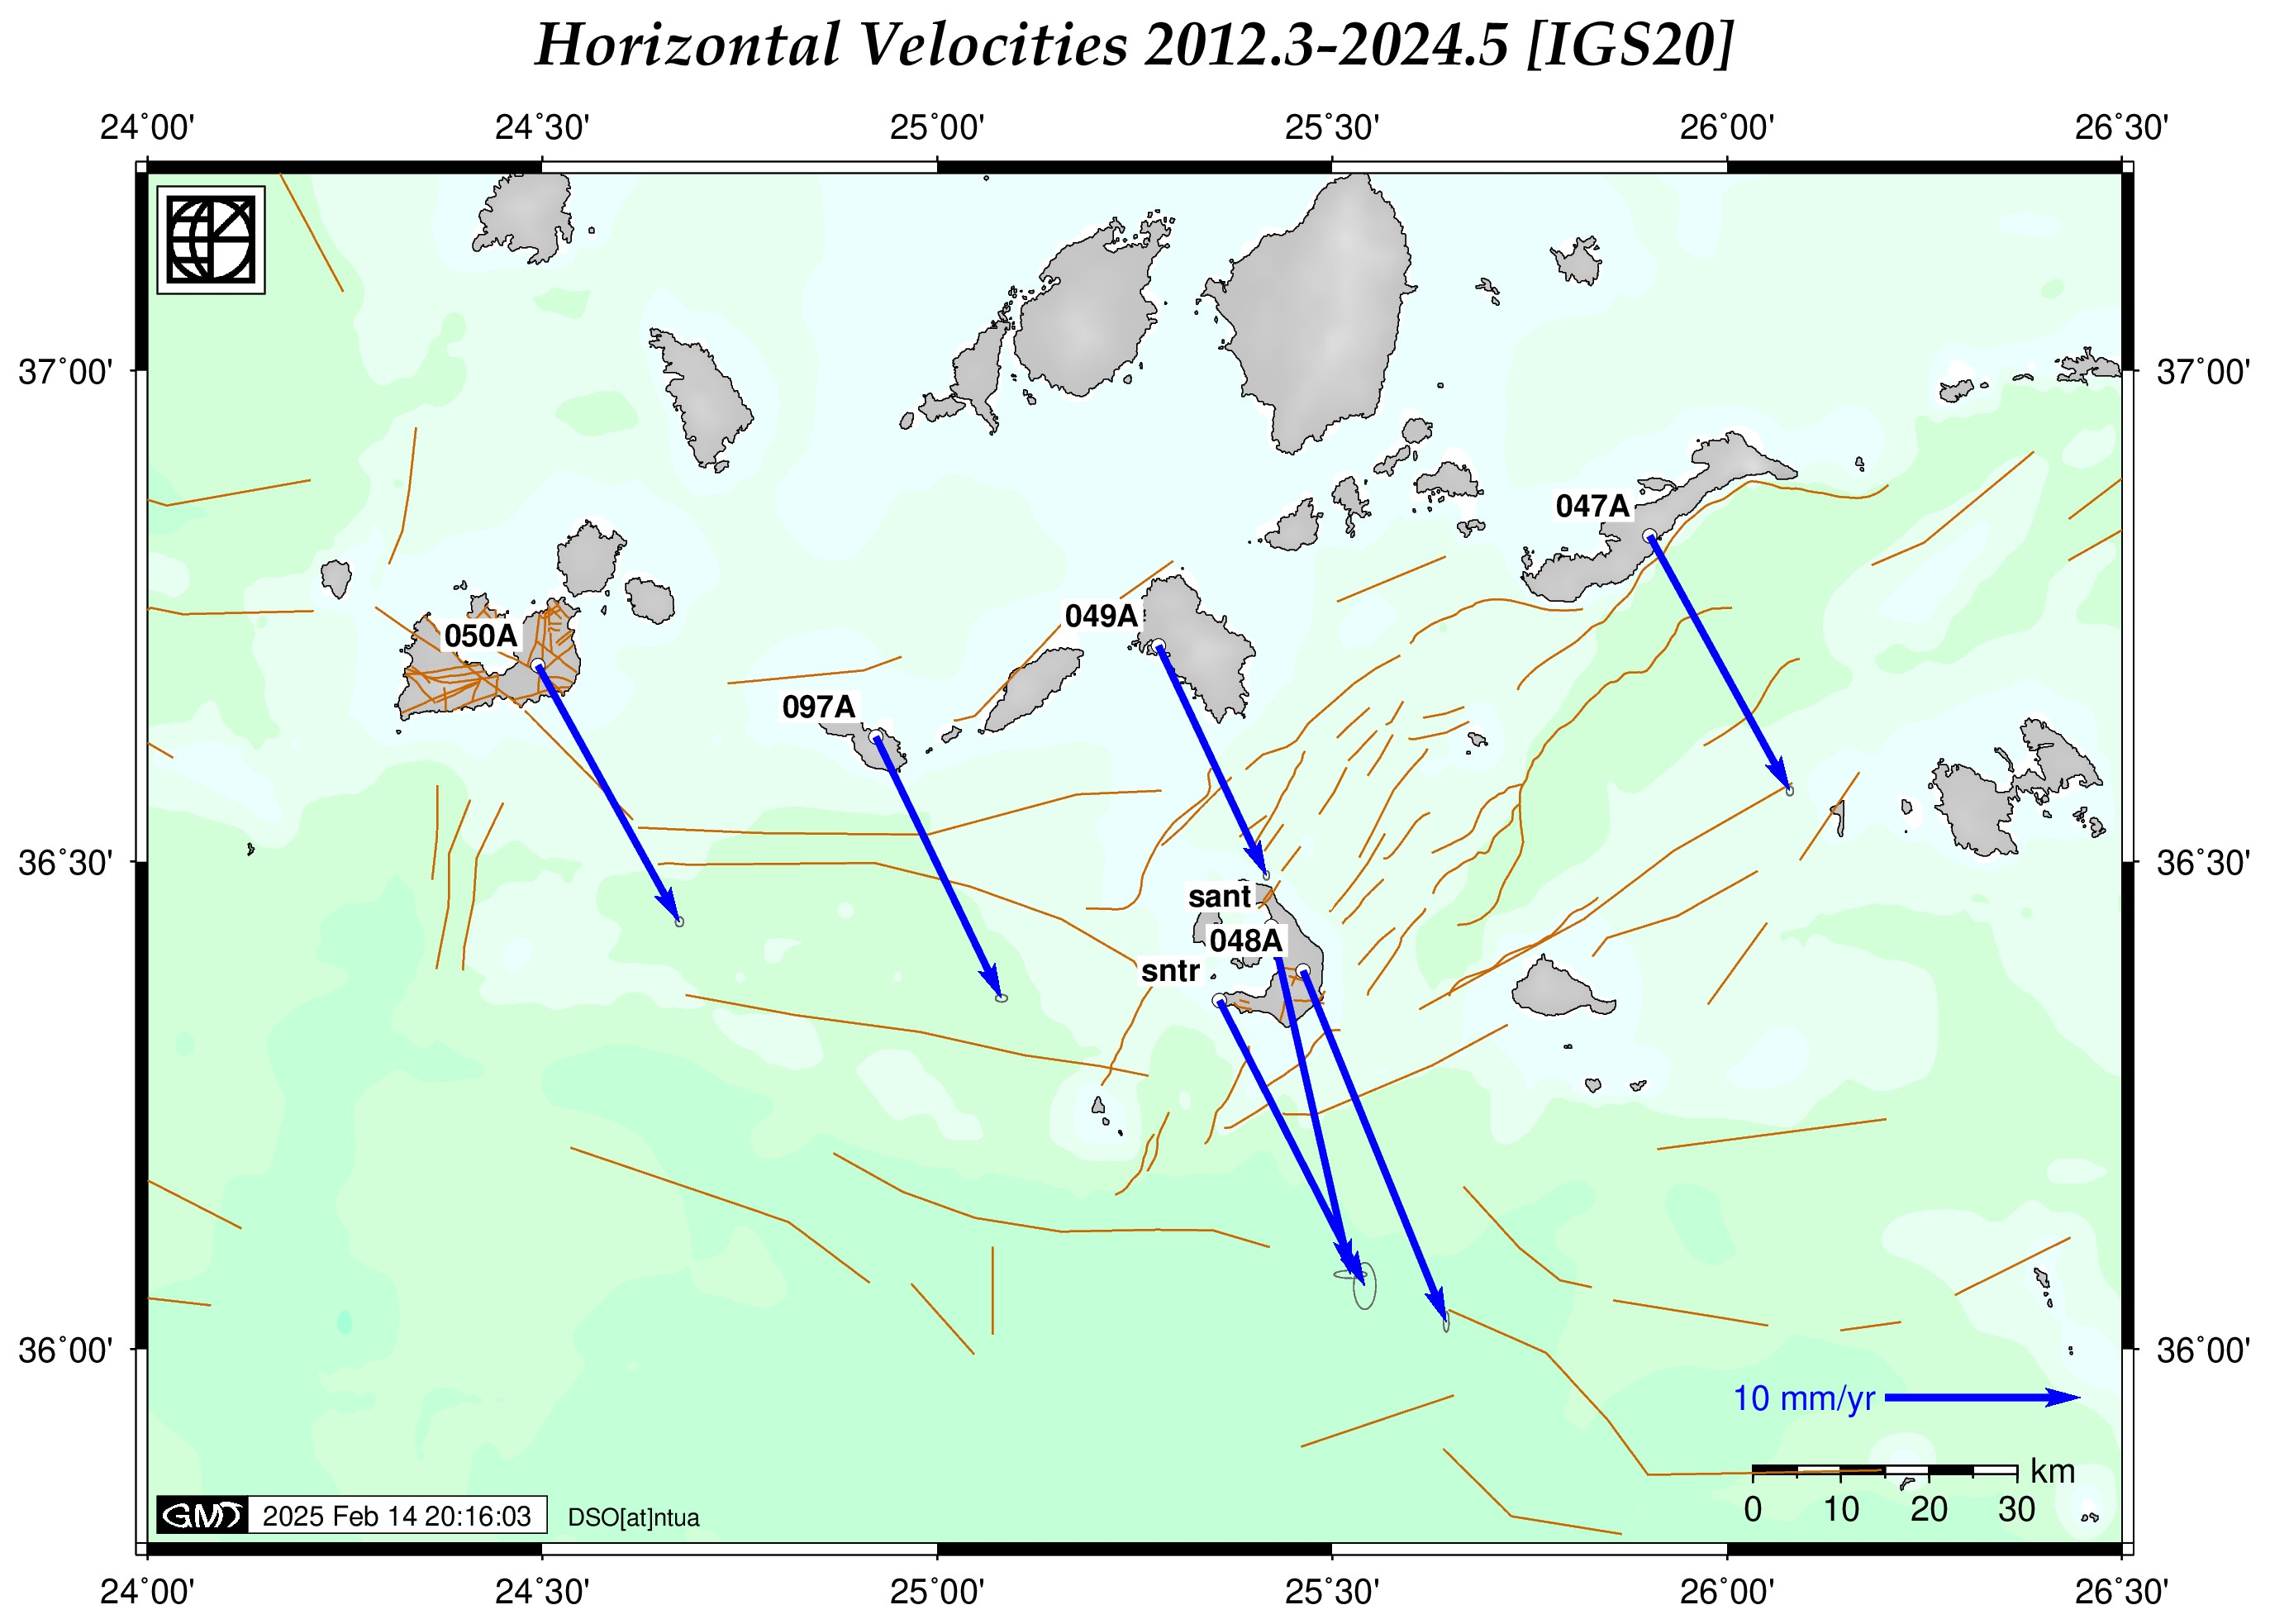
\includegraphics[width=.97\textwidth]{sant_1224_vhor.jpg}
      \end{center}  
    \end{column}
    \begin{column}{.5\textwidth}
      \begin{center}
        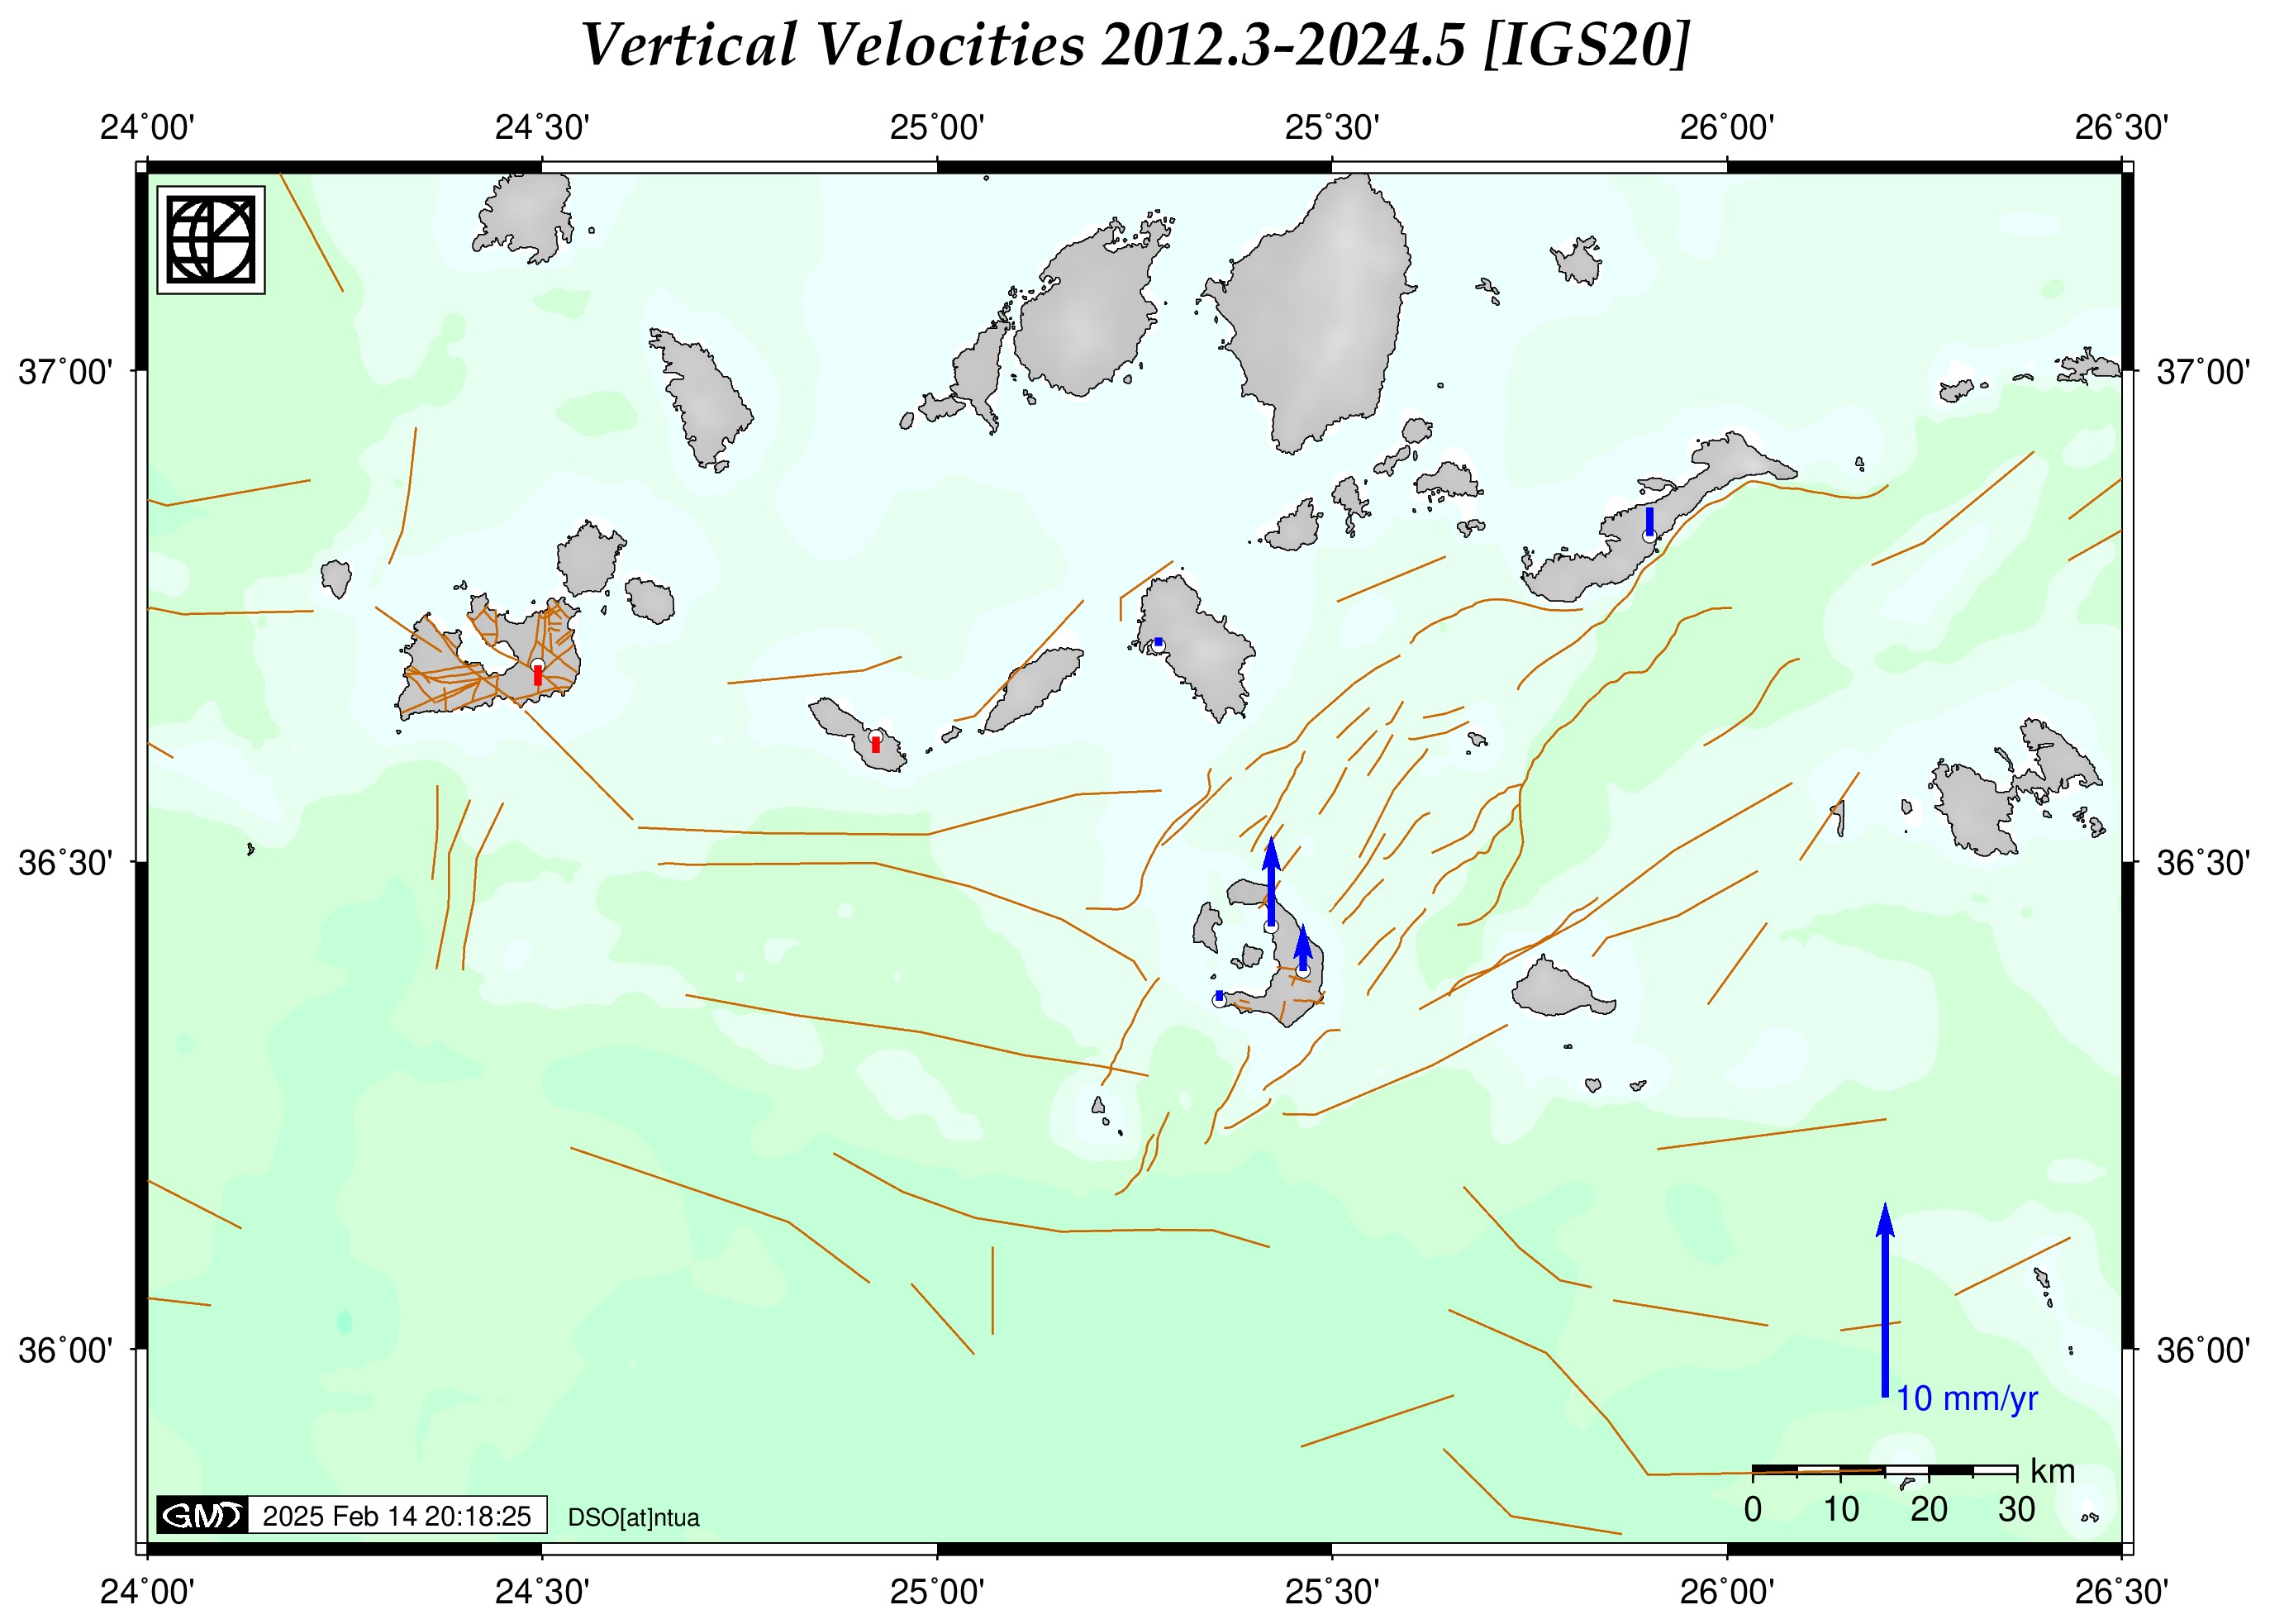
\includegraphics[width=.97\textwidth]{sant_1224_vver.jpg}
      \end{center}       
    \end{column}
  \end{columns}
~\\[1em]   
  \begin{tiny}
  \begin{itemize}\setlength\itemsep{.1em}
    \item[*] Δημιουργία χαρτών: Generic Mapping Tools \citep{gmt}
    \item[*] Υπόβαθρο: ETOPO1 \citep{etopo1}
    \item[*] Βάση ρηγμάτων: NOAfaults v6.0 \citep{noafaults}
  \end{itemize}
  \end{tiny}  
 
\end{frame}
\note{}

 % ------------------------------------------------------------------------------
\begin{frame}
  \frametitle{Ανάλυση χρονοσειρών}
  \framesubtitle{}
  \label{}
  \vskip-1cm
  \begin{columns}[T]
    \begin{column}{.25\textwidth}
      \begin{center}
      {\scriptsize 047A (Αμοργός)}
        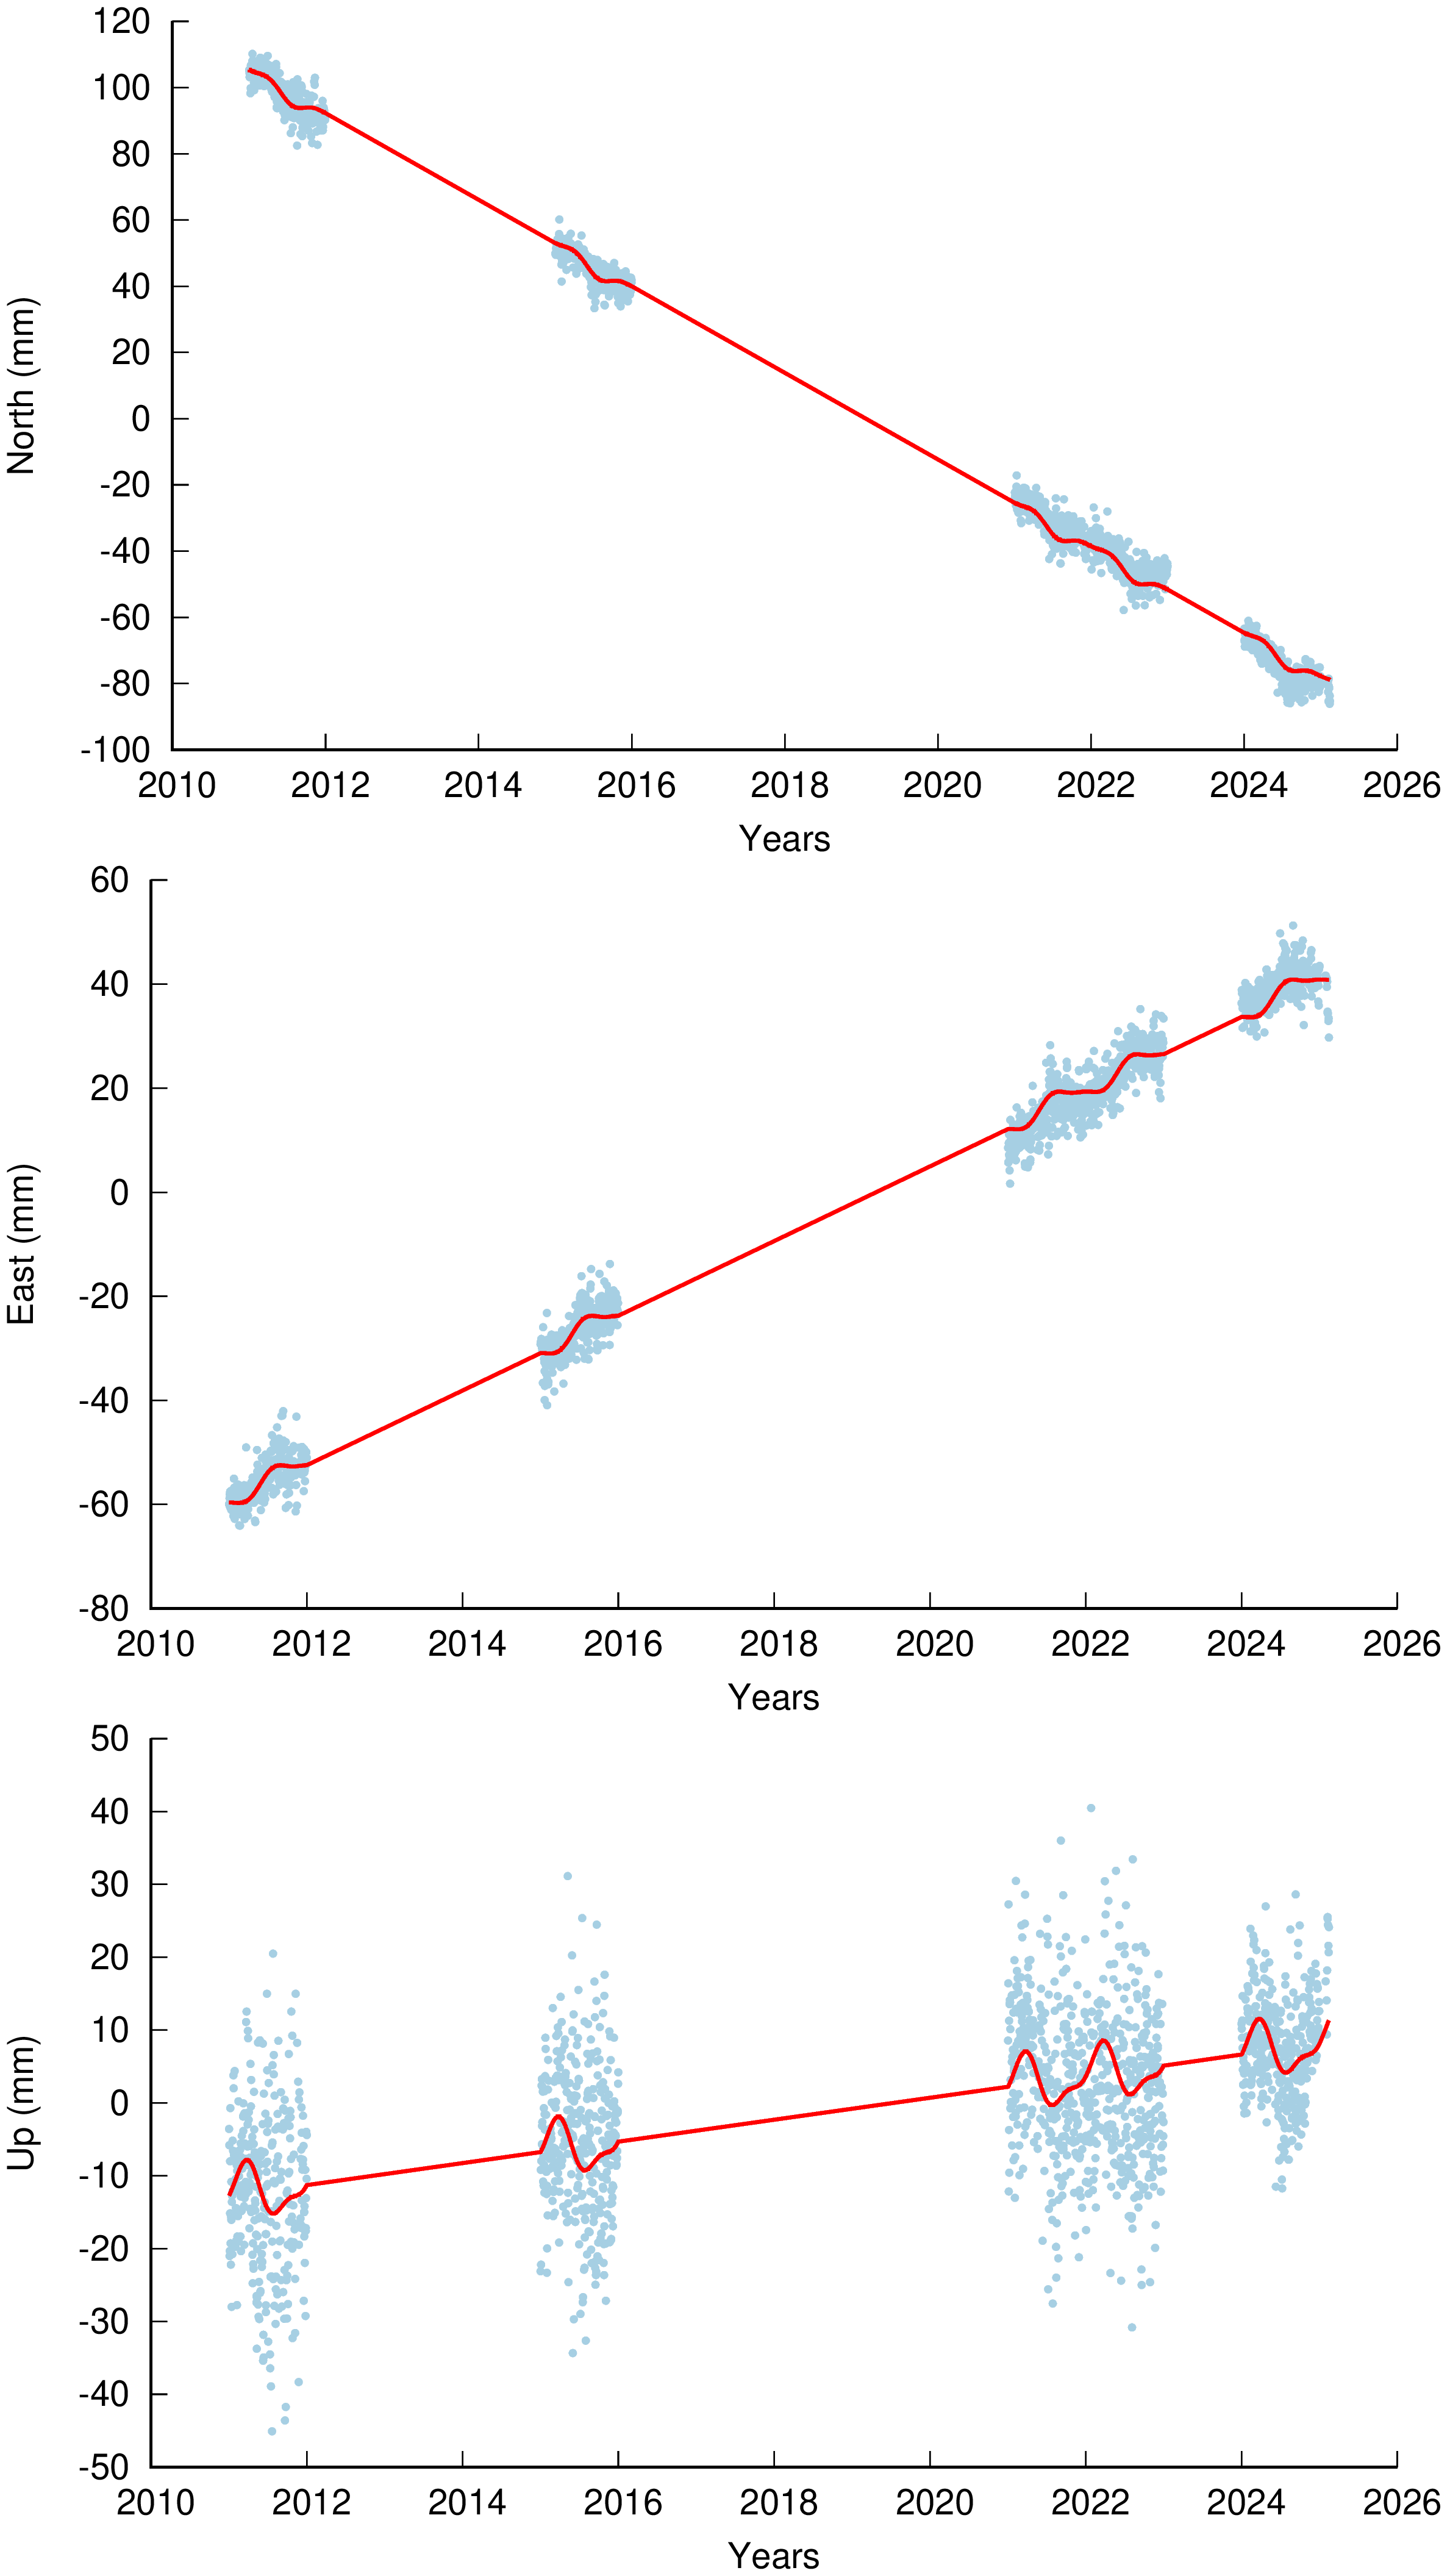
\includegraphics[width=.97\textwidth]{047a-mod.png}
      \end{center}  
    \end{column}
    \begin{column}{.25\textwidth}
      \begin{center}
       {\scriptsize 049A (Ίος)}
        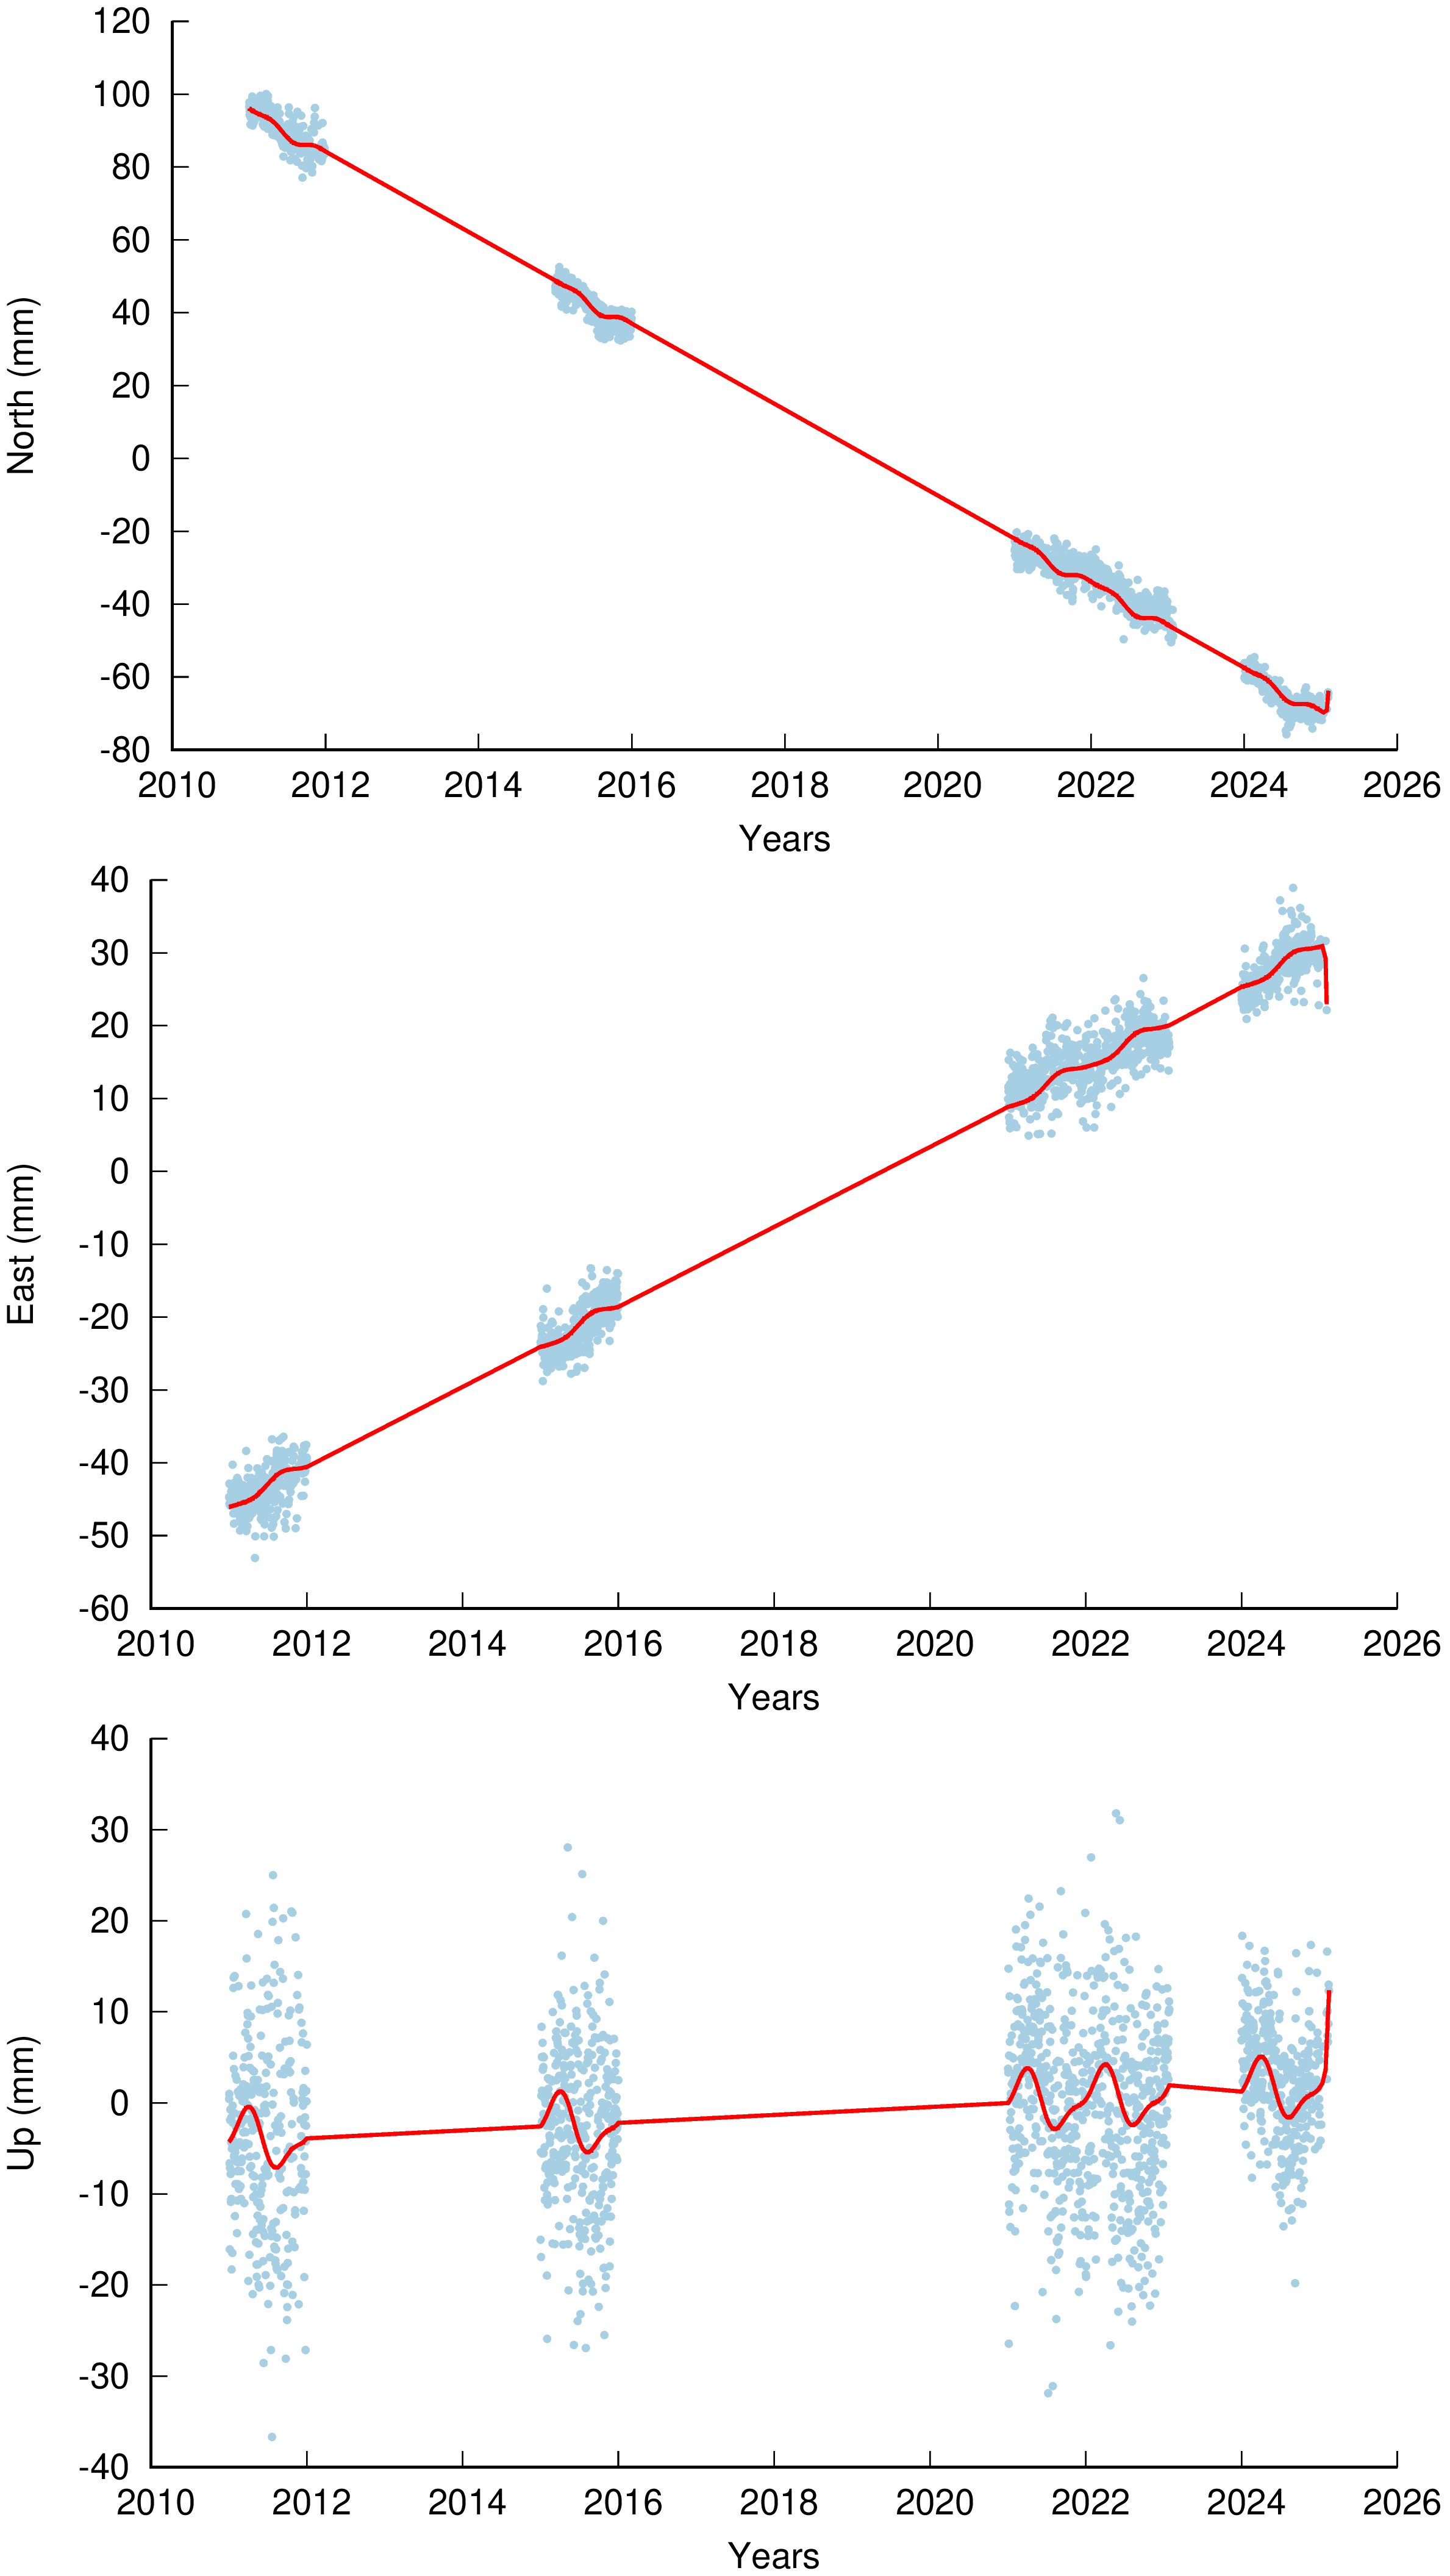
\includegraphics[width=.97\textwidth]{049a-mod.png}
      \end{center}       
    \end{column}
  \begin{column}{.25\textwidth}
      \begin{center}
       {\scriptsize 048A (Θήρα)}
        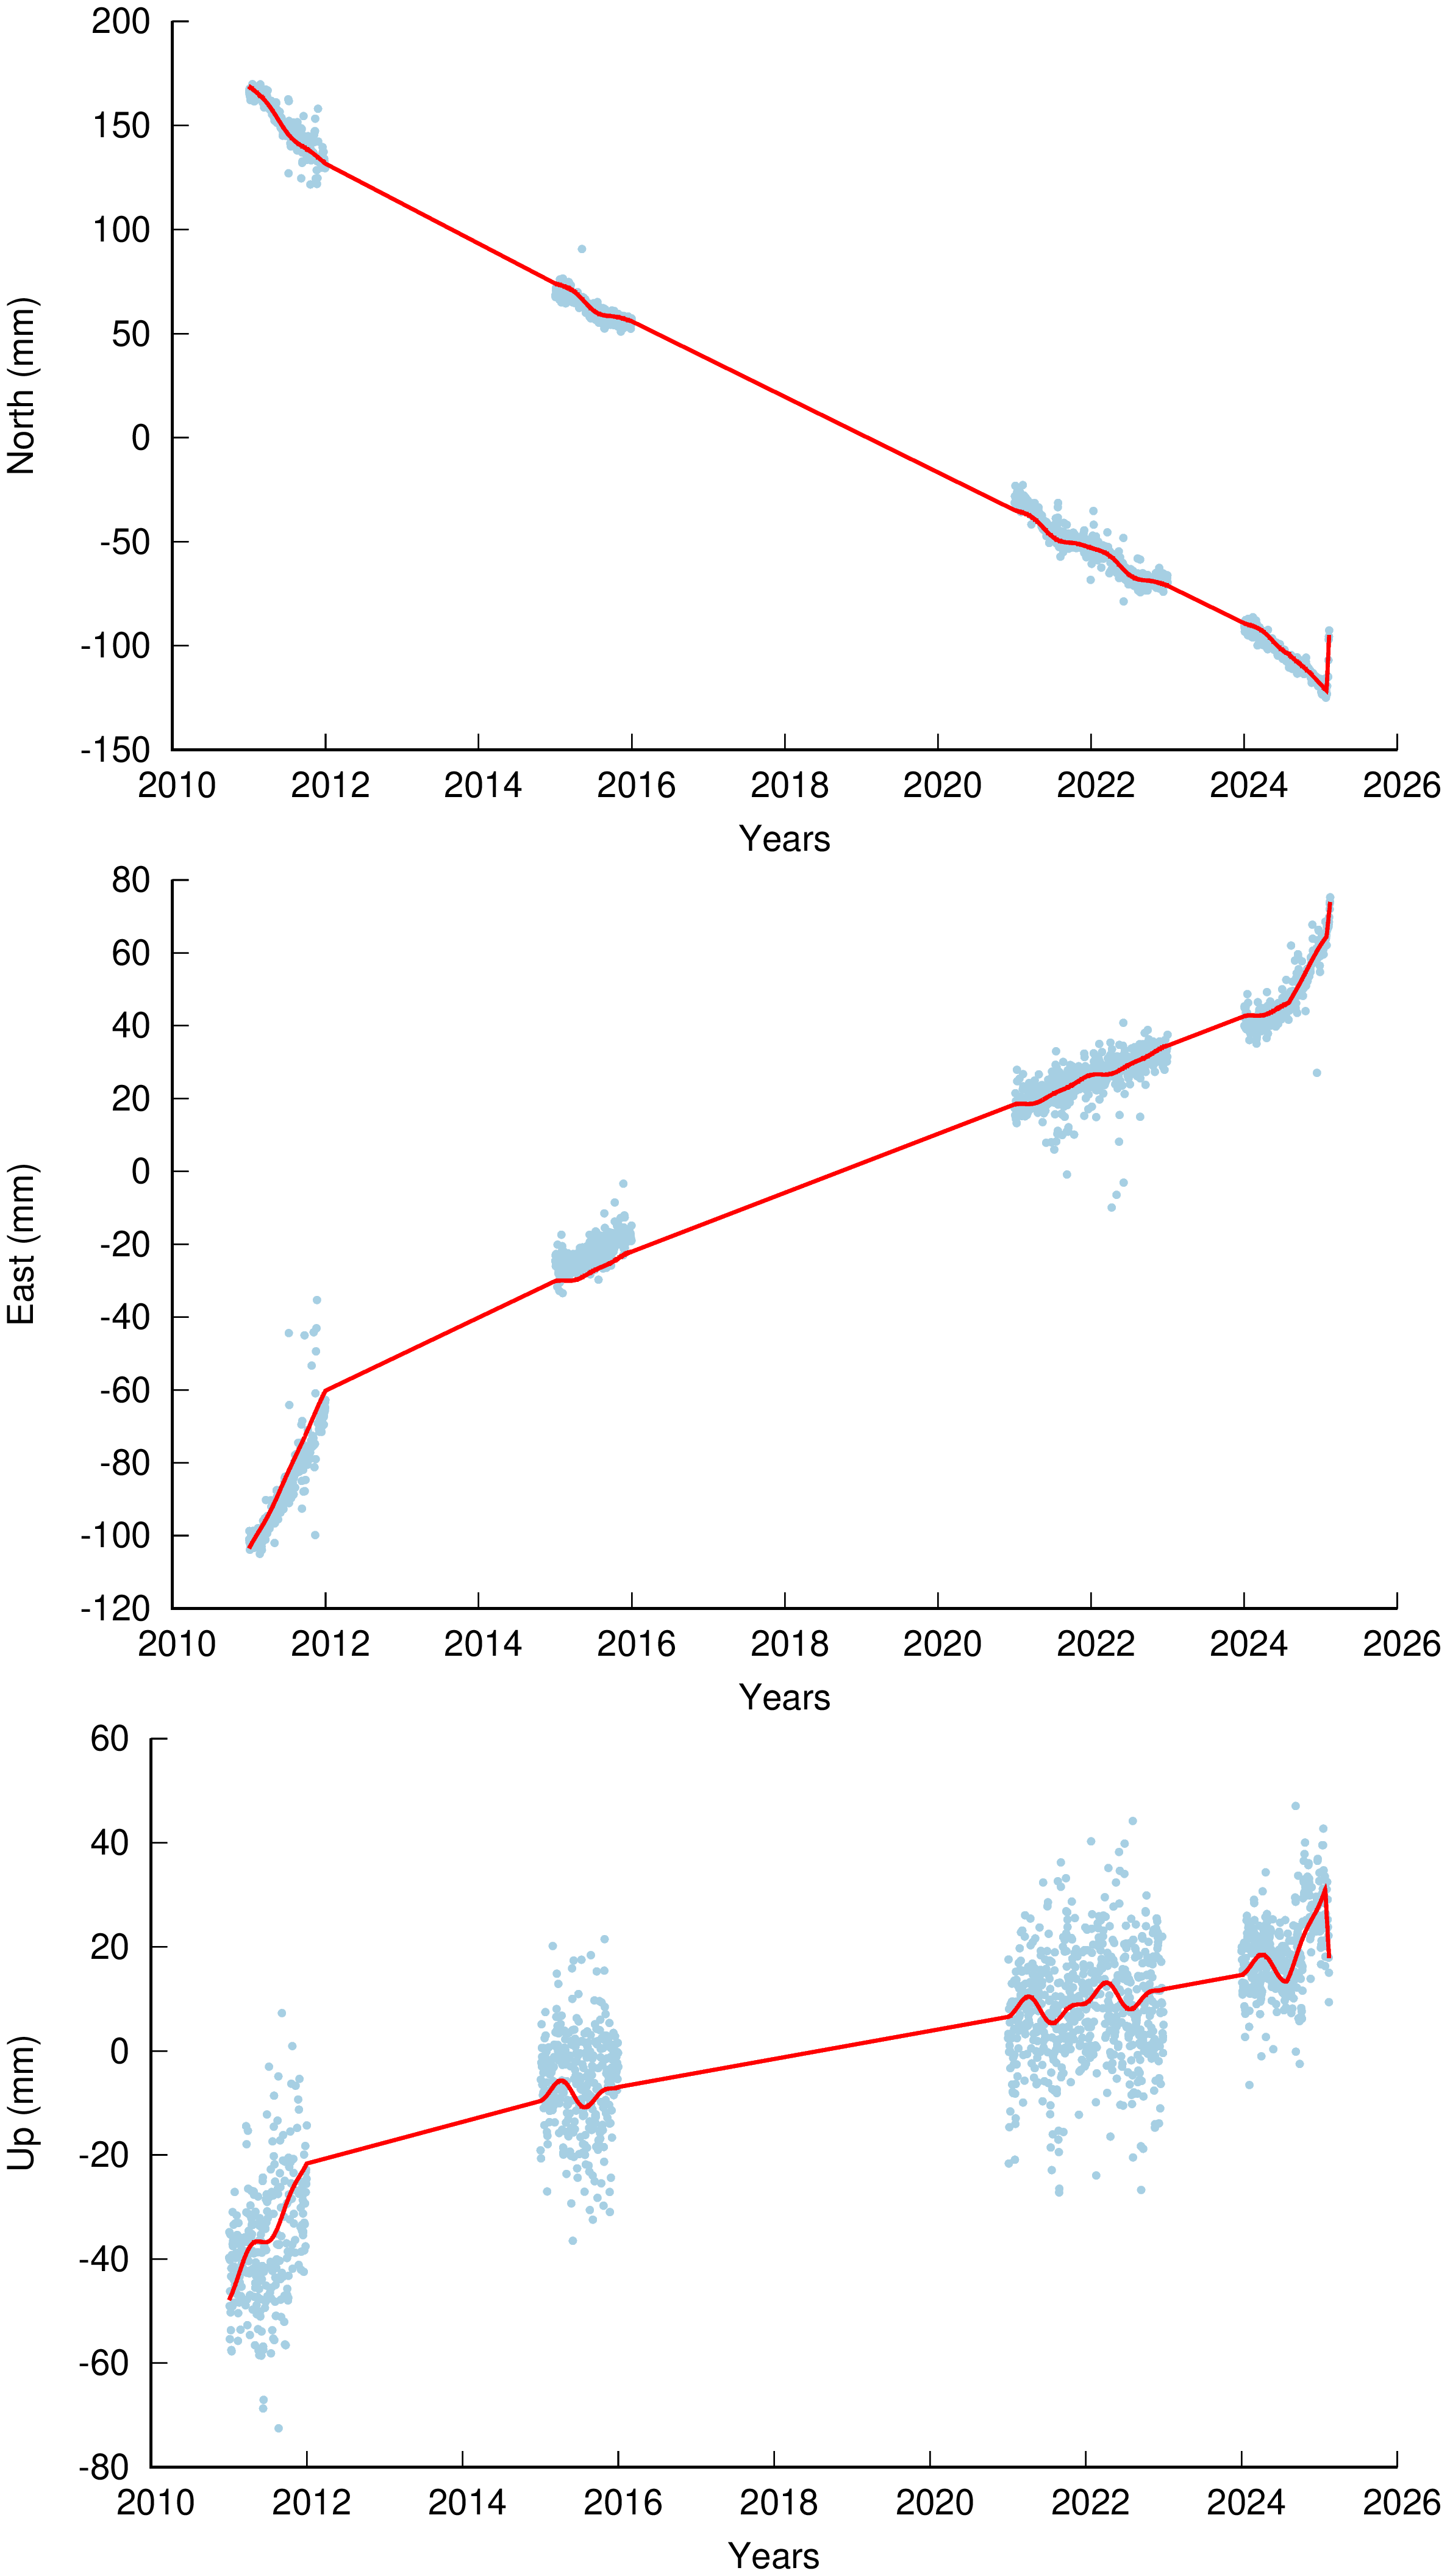
\includegraphics[width=.97\textwidth]{048a-mod.png}
      \end{center}  
    \end{column}
    \begin{column}{.25\textwidth}
      \begin{center}
       {\scriptsize SNTR (Φάρος)}
        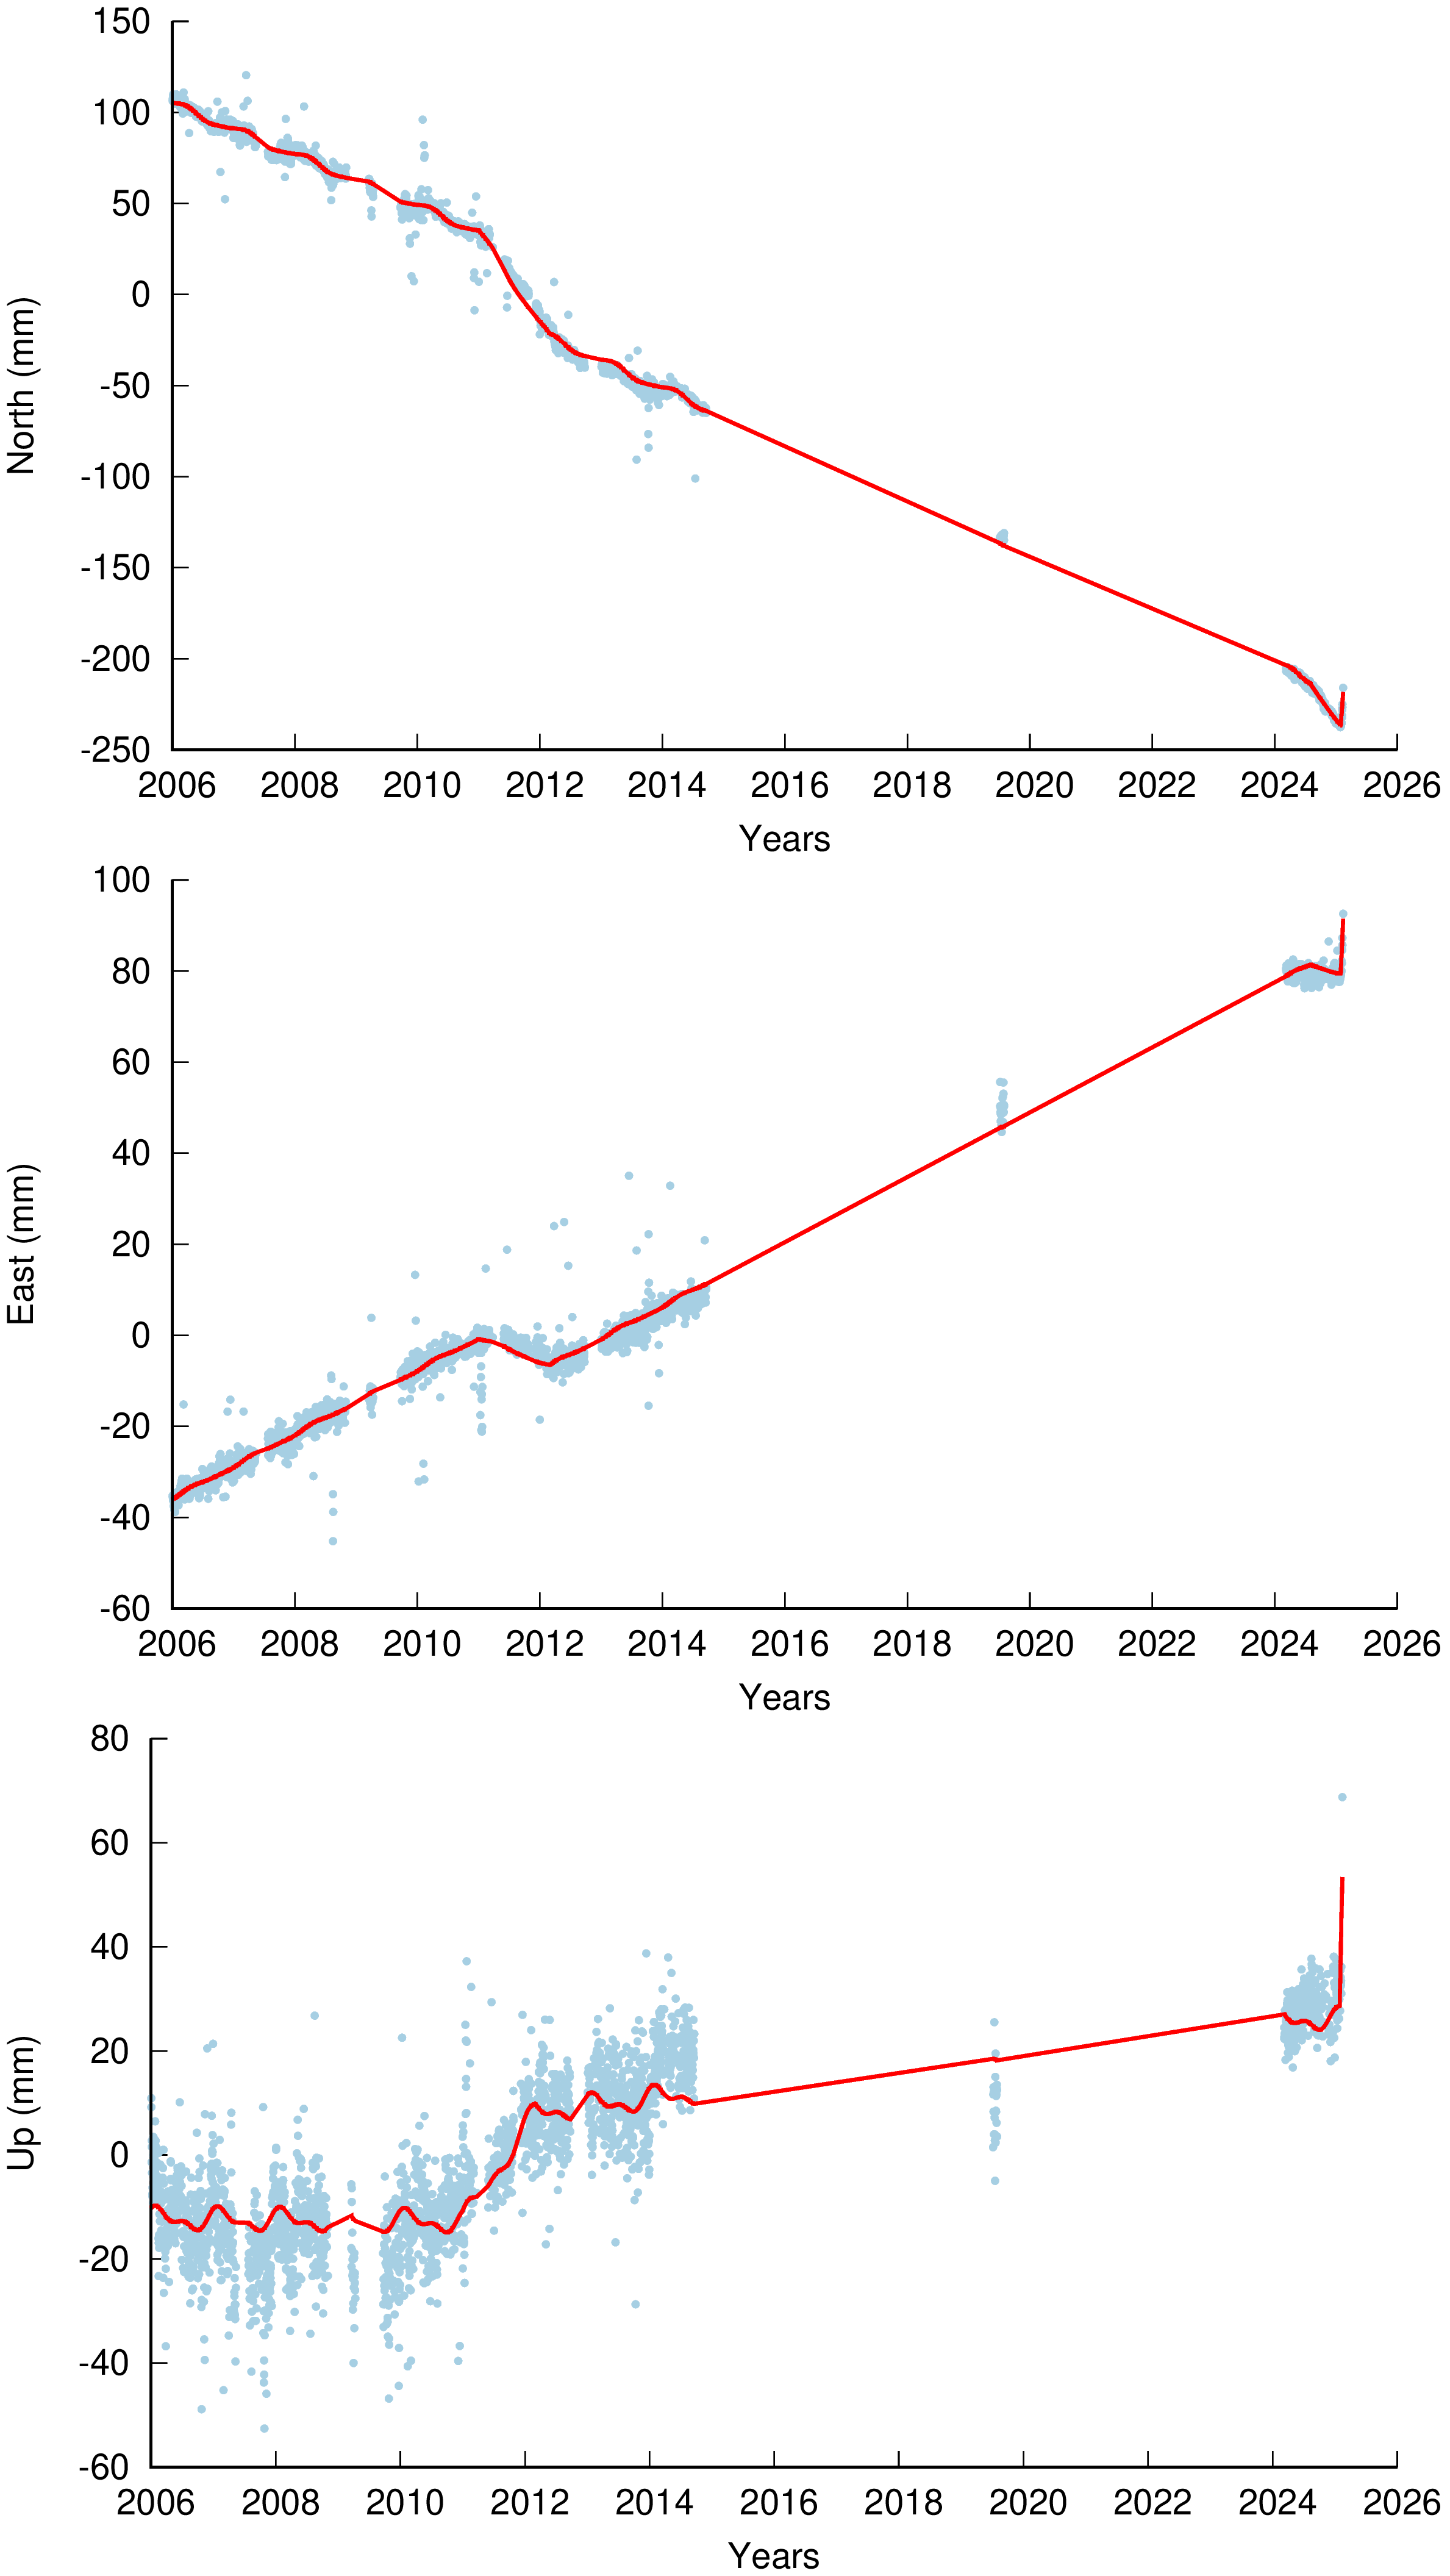
\includegraphics[width=.97\textwidth]{sntr-mod.png}
      \end{center}       
    \end{column}
  \end{columns}  
  
\end{frame}
\note{}

 % ------------------------------------------------------------------------------
\begin{frame}
  \frametitle{Μετακινήσεις 2024.6 - 2025.1 }
  \framesubtitle{}
  \label{}
  \vskip-.5cm
  \begin{columns}[T]
    \begin{column}{.5\textwidth}
      \begin{center}
        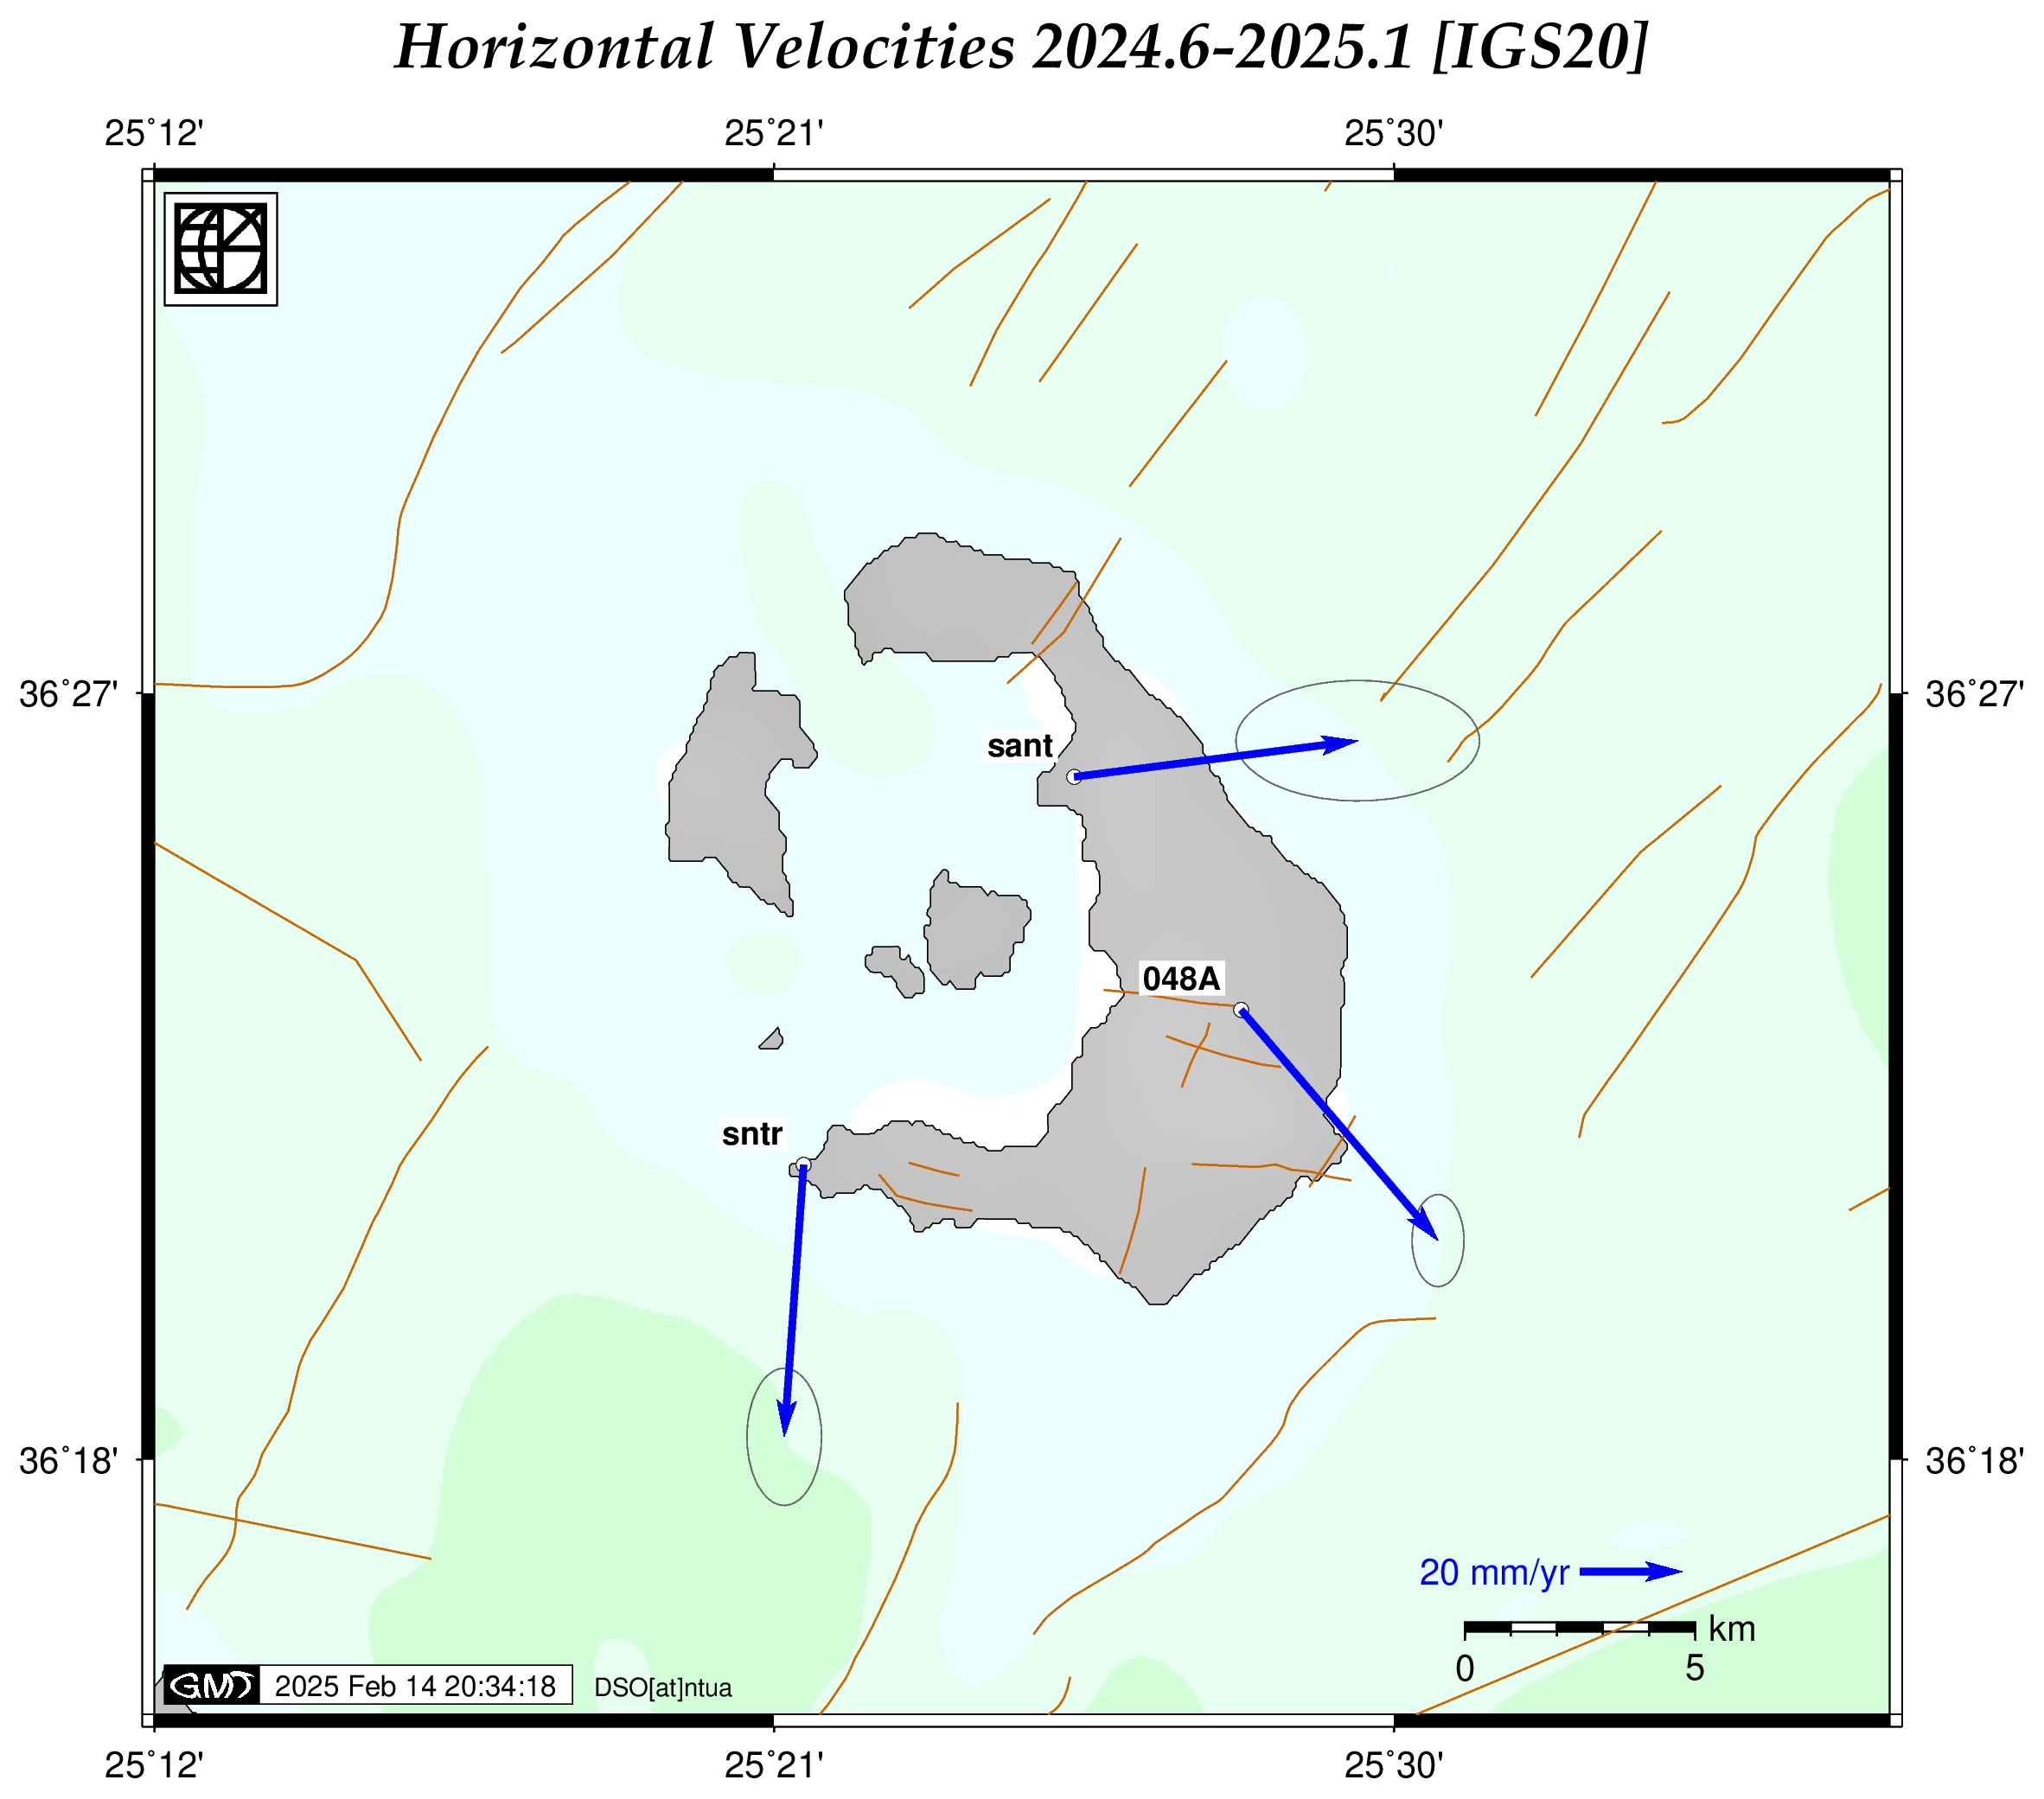
\includegraphics[width=.97\textwidth]{sant_2425_vhor.jpg}
      \end{center}  
    \end{column}
    \begin{column}{.5\textwidth}
      \begin{center}
        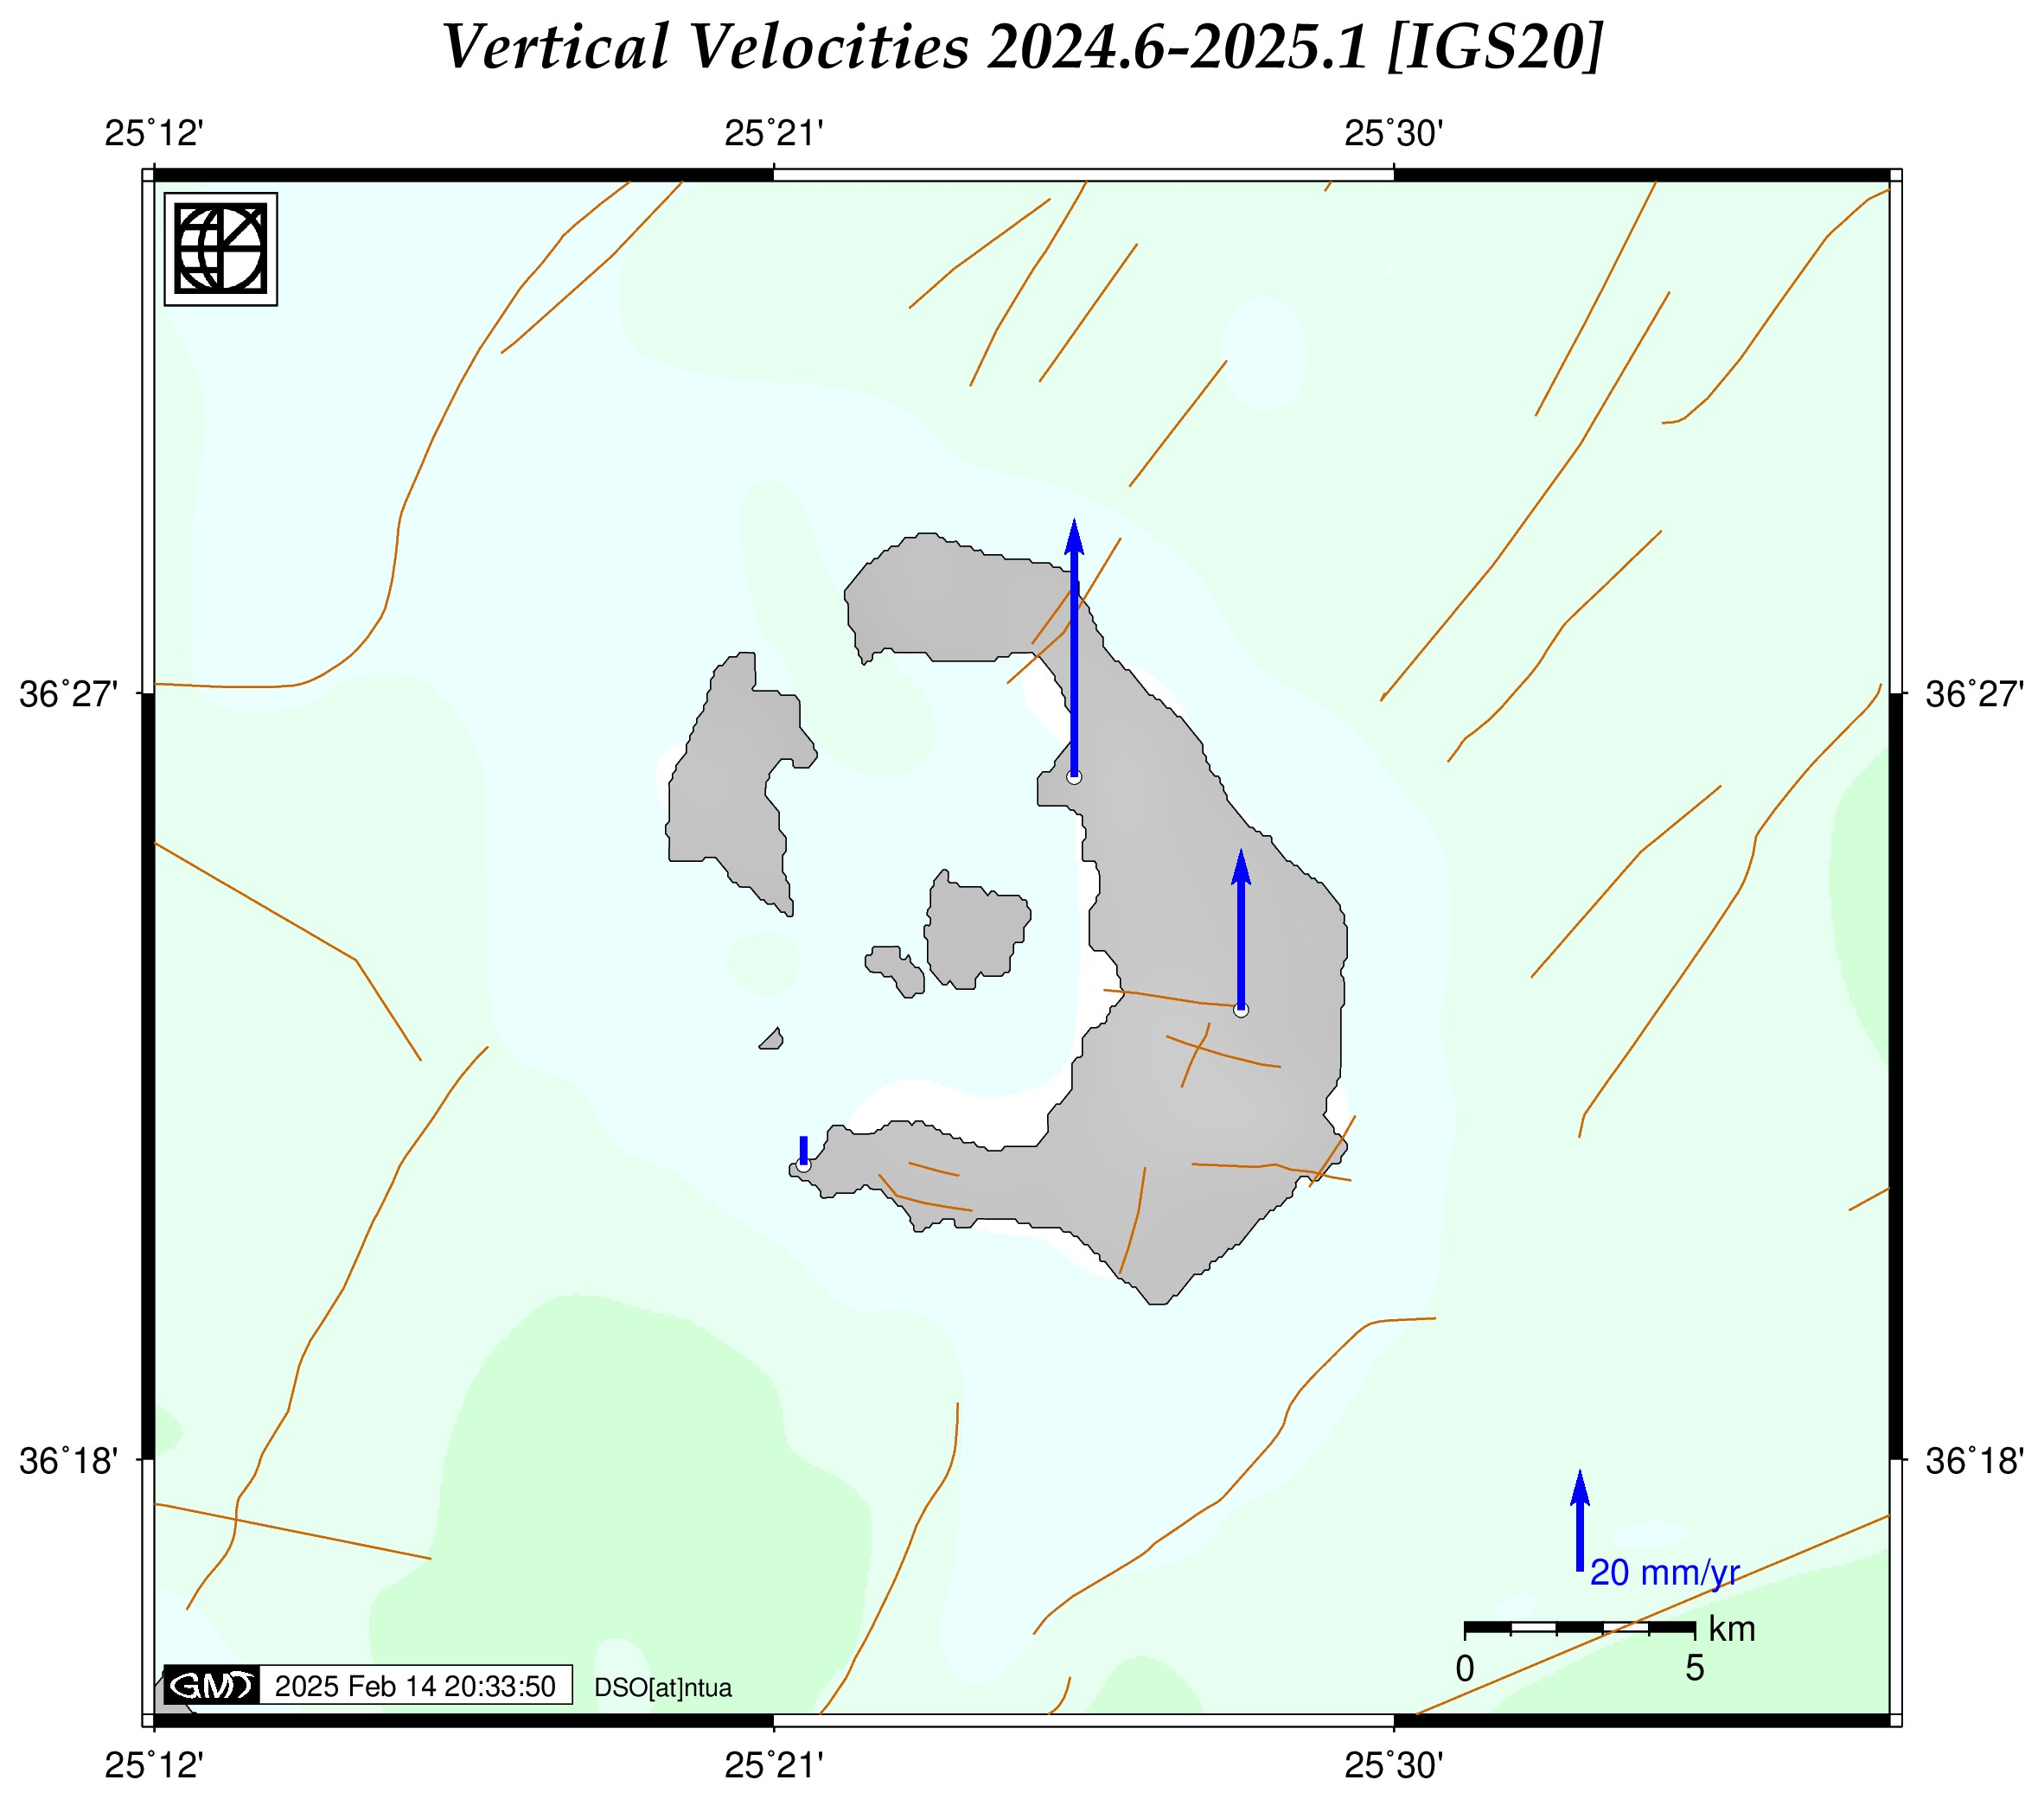
\includegraphics[width=.97\textwidth]{sant_2425_vver.jpg}
      \end{center}       
    \end{column}
  \end{columns}  

\end{frame}
\note{}



 % ------------------------------------------------------------------------------
\begin{frame}
  \frametitle{Ανάλυση χρονοσειρών}
  \framesubtitle{}
  \label{}
  \vskip-1cm
  \begin{columns}[T]
    \begin{column}{.25\textwidth}
      \begin{center}
      {\scriptsize 047A (Αμοργός)}
        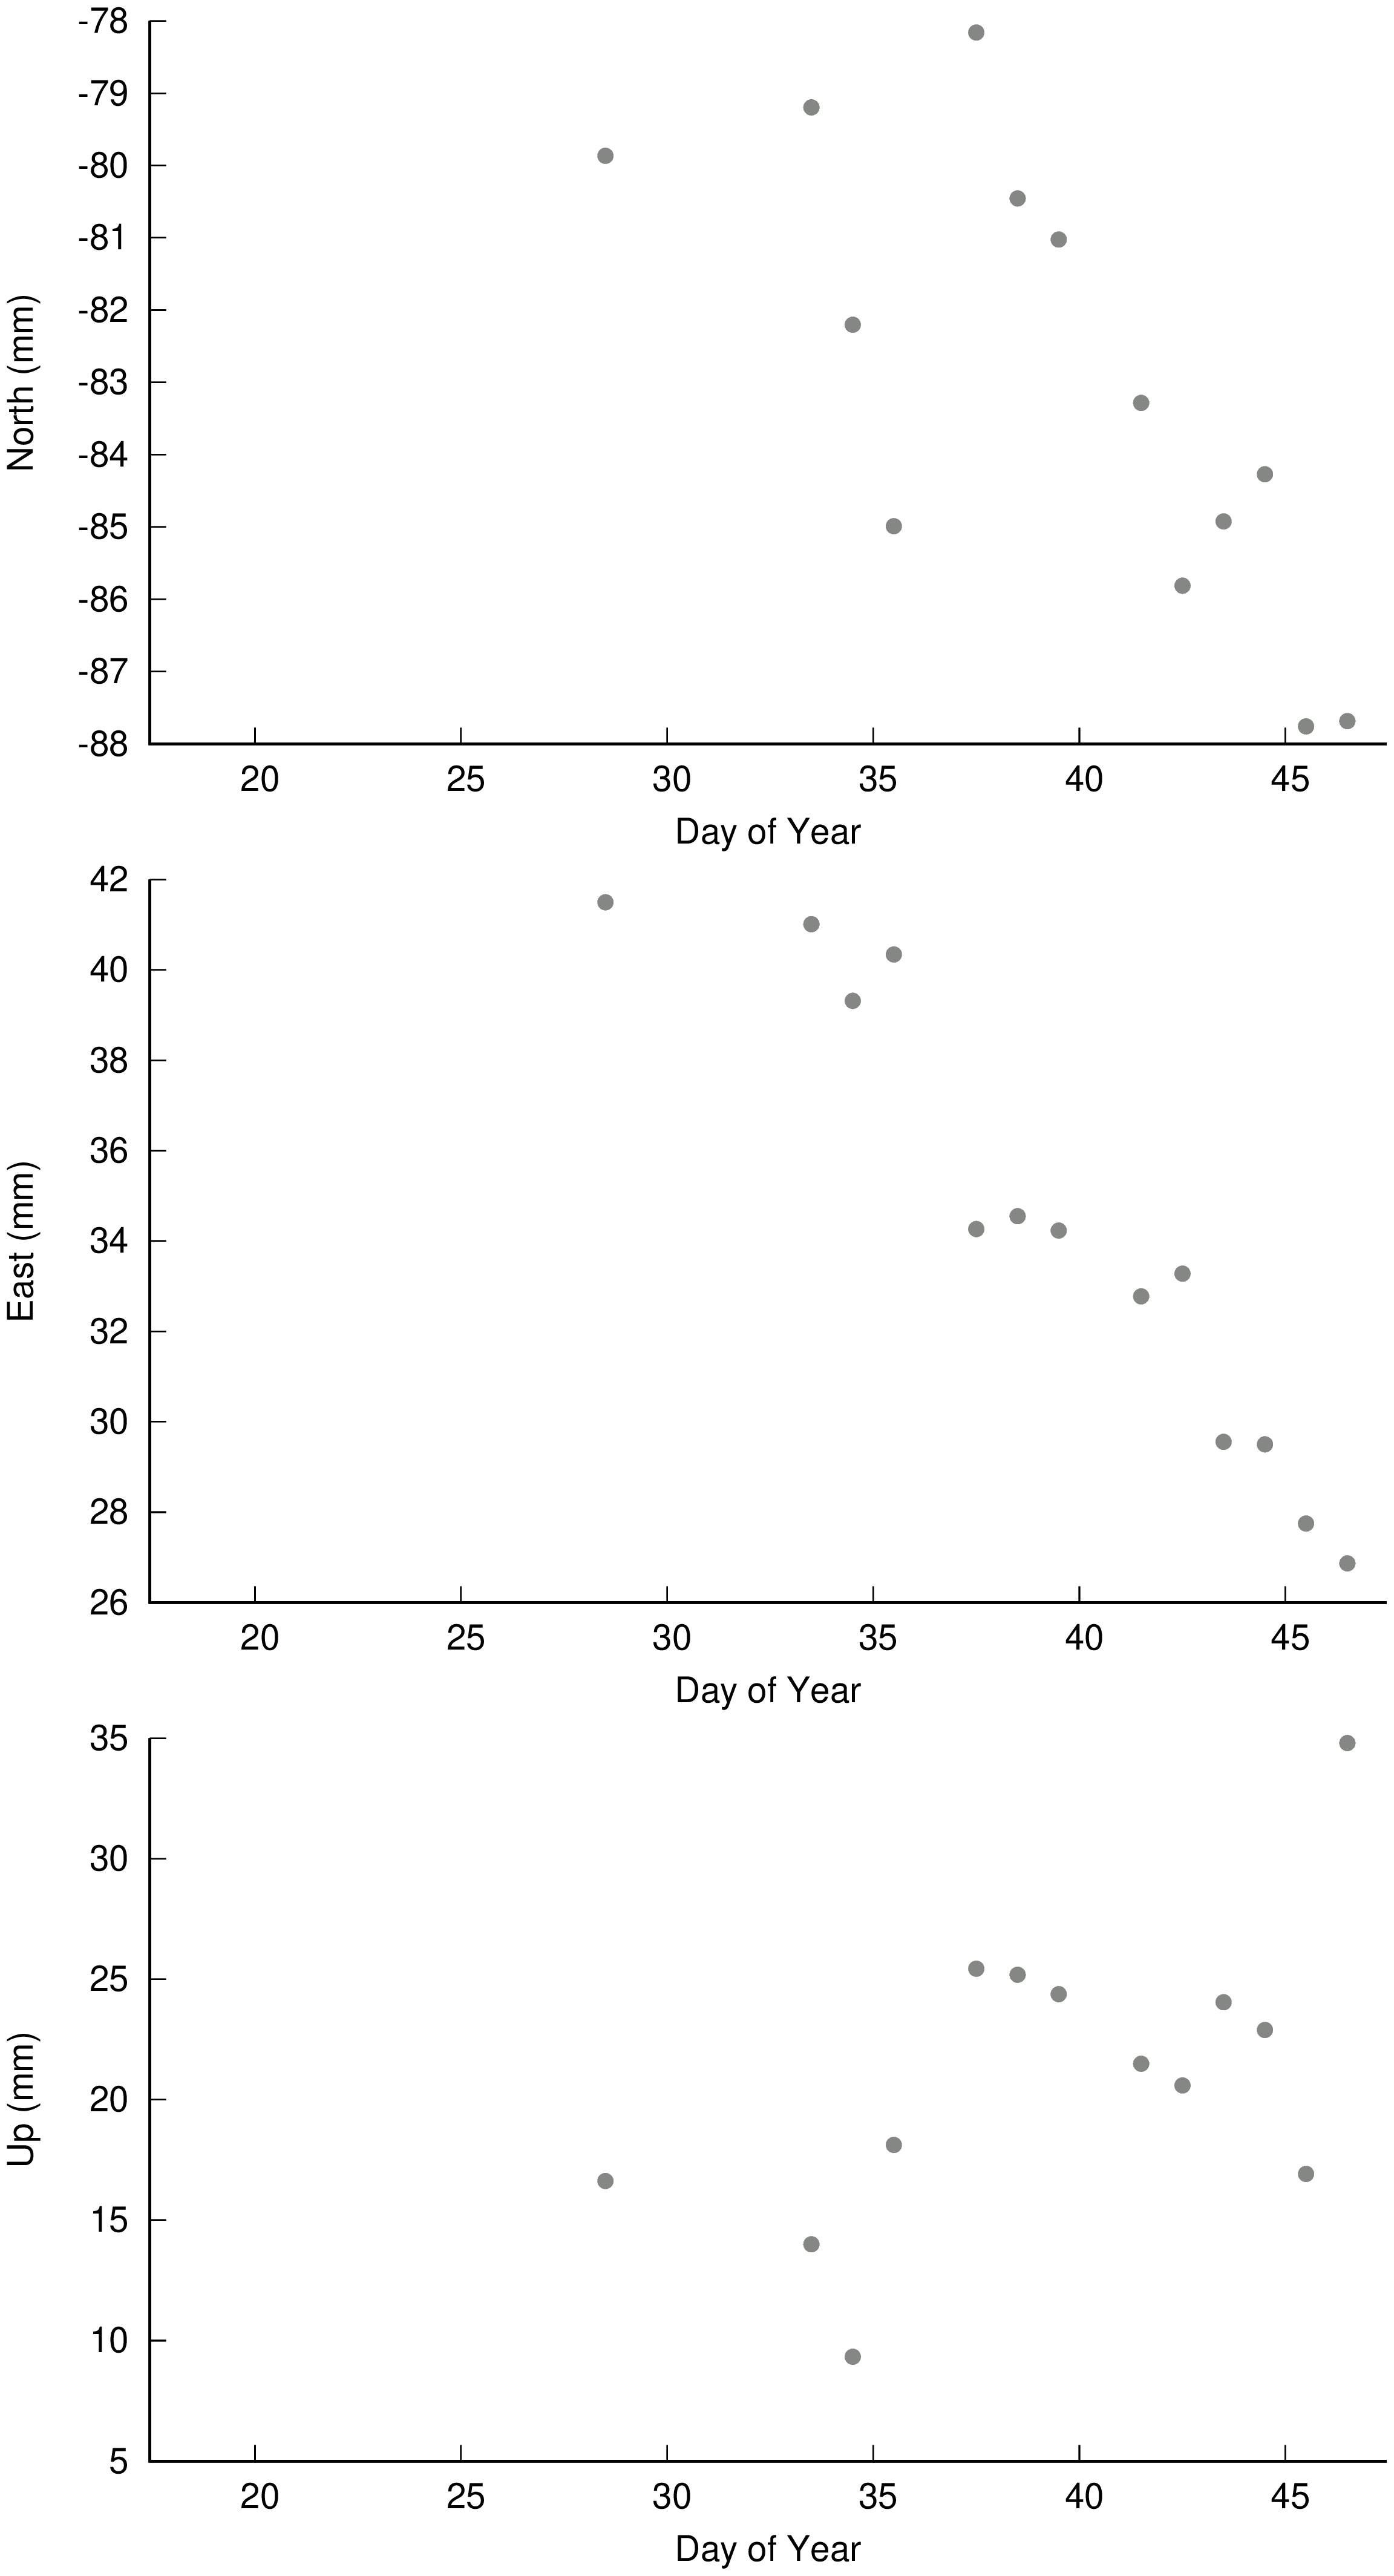
\includegraphics[width=.97\textwidth]{047a-lmn.png}
      \end{center}  
    \end{column}
    \begin{column}{.25\textwidth}
      \begin{center}
       {\scriptsize 049A (Ίος)}
        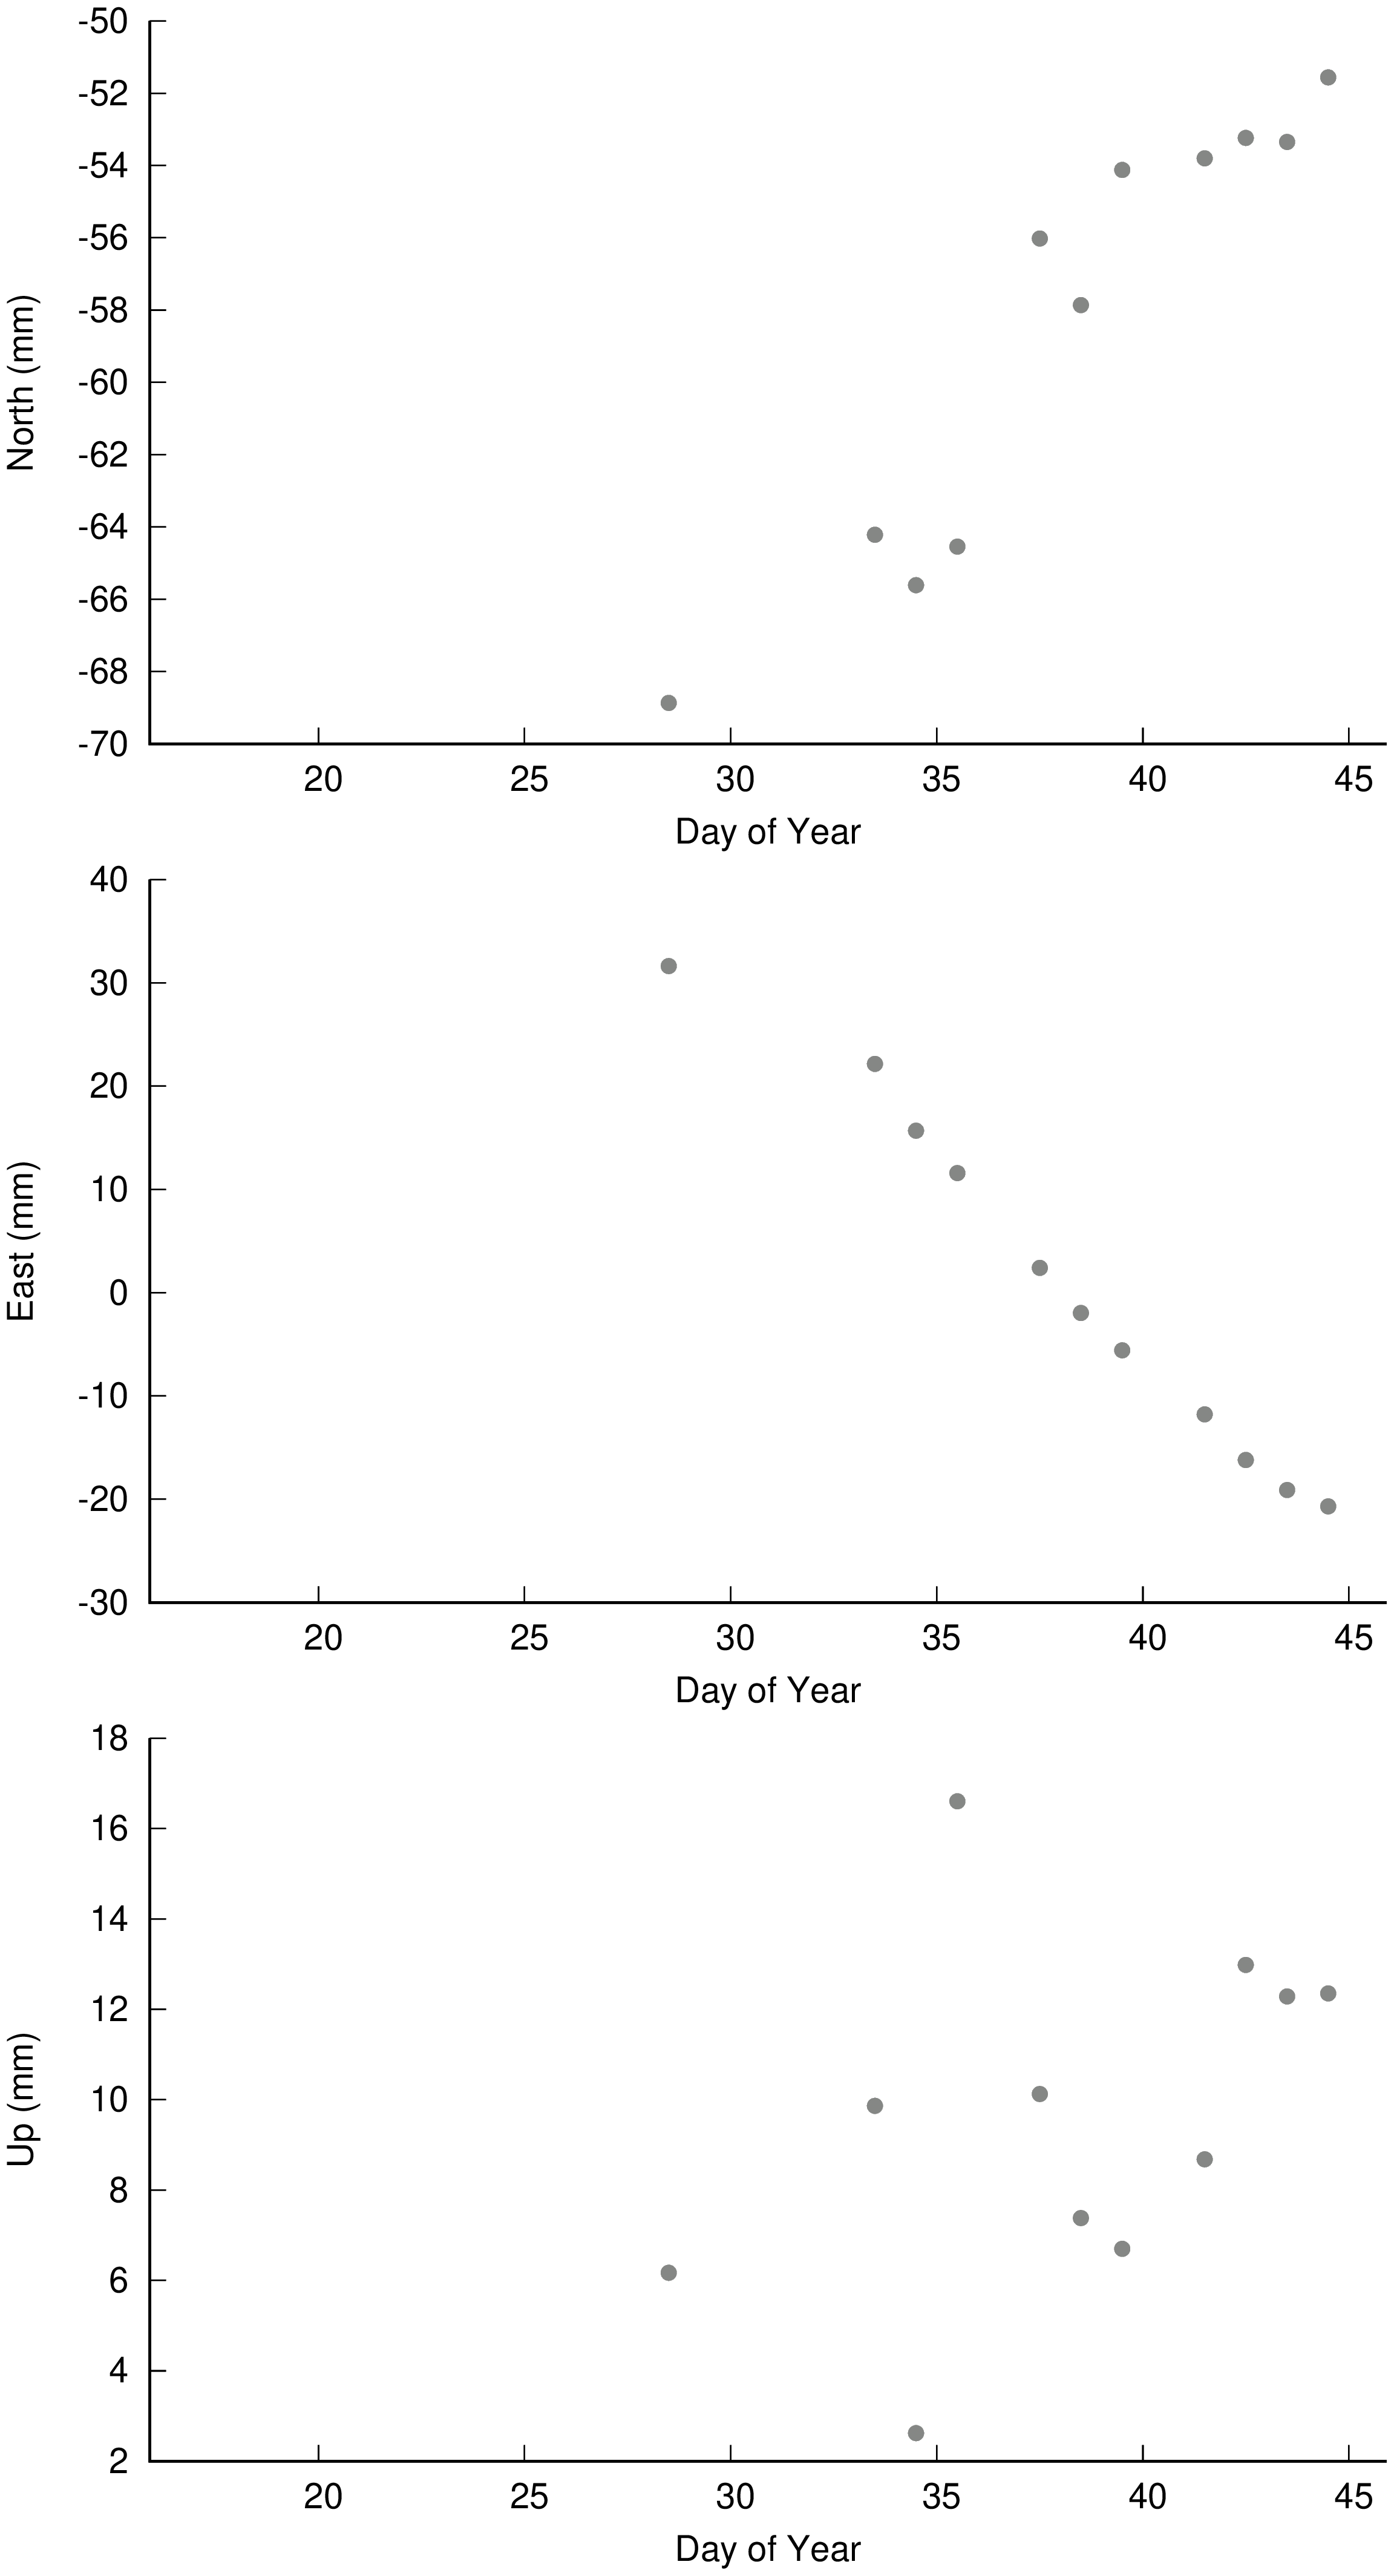
\includegraphics[width=.97\textwidth]{049a-lmn.png}
      \end{center}       
    \end{column}
  \begin{column}{.25\textwidth}
      \begin{center}
       {\scriptsize 048A (Θήρα)}
        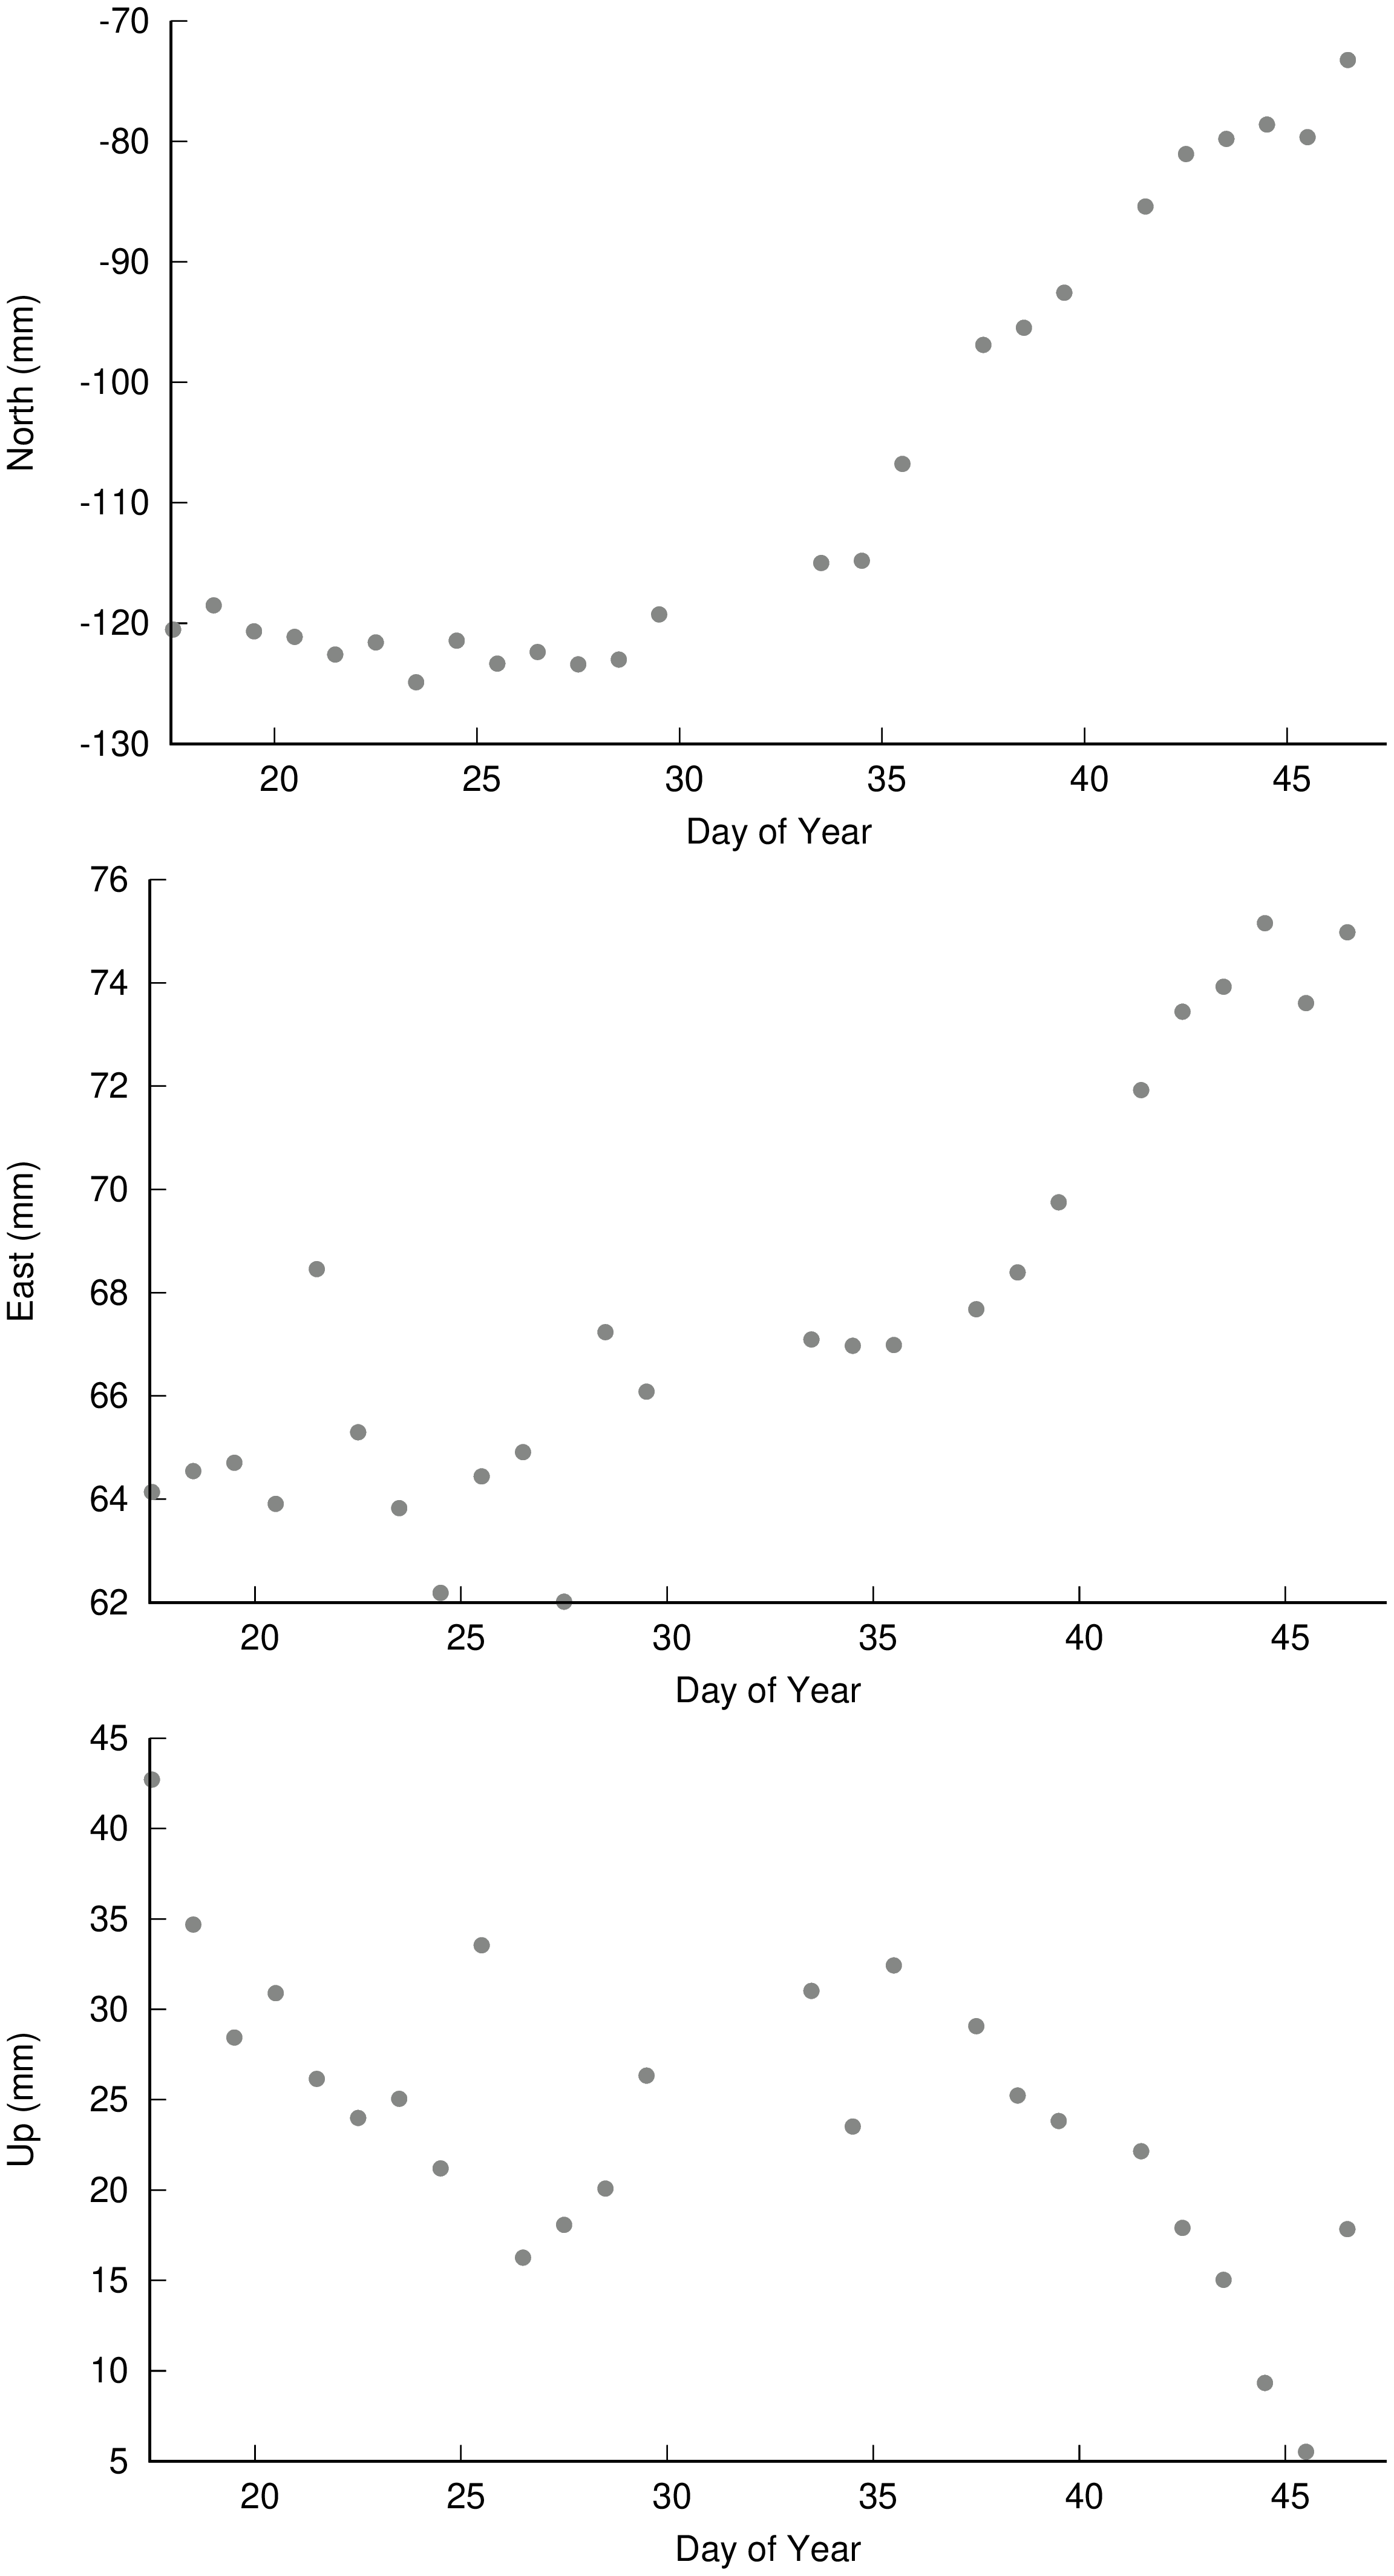
\includegraphics[width=.97\textwidth]{048a-lmn.png}
      \end{center}  
    \end{column}
    \begin{column}{.25\textwidth}
      \begin{center}
       {\scriptsize SNTR (Φάρος)}
        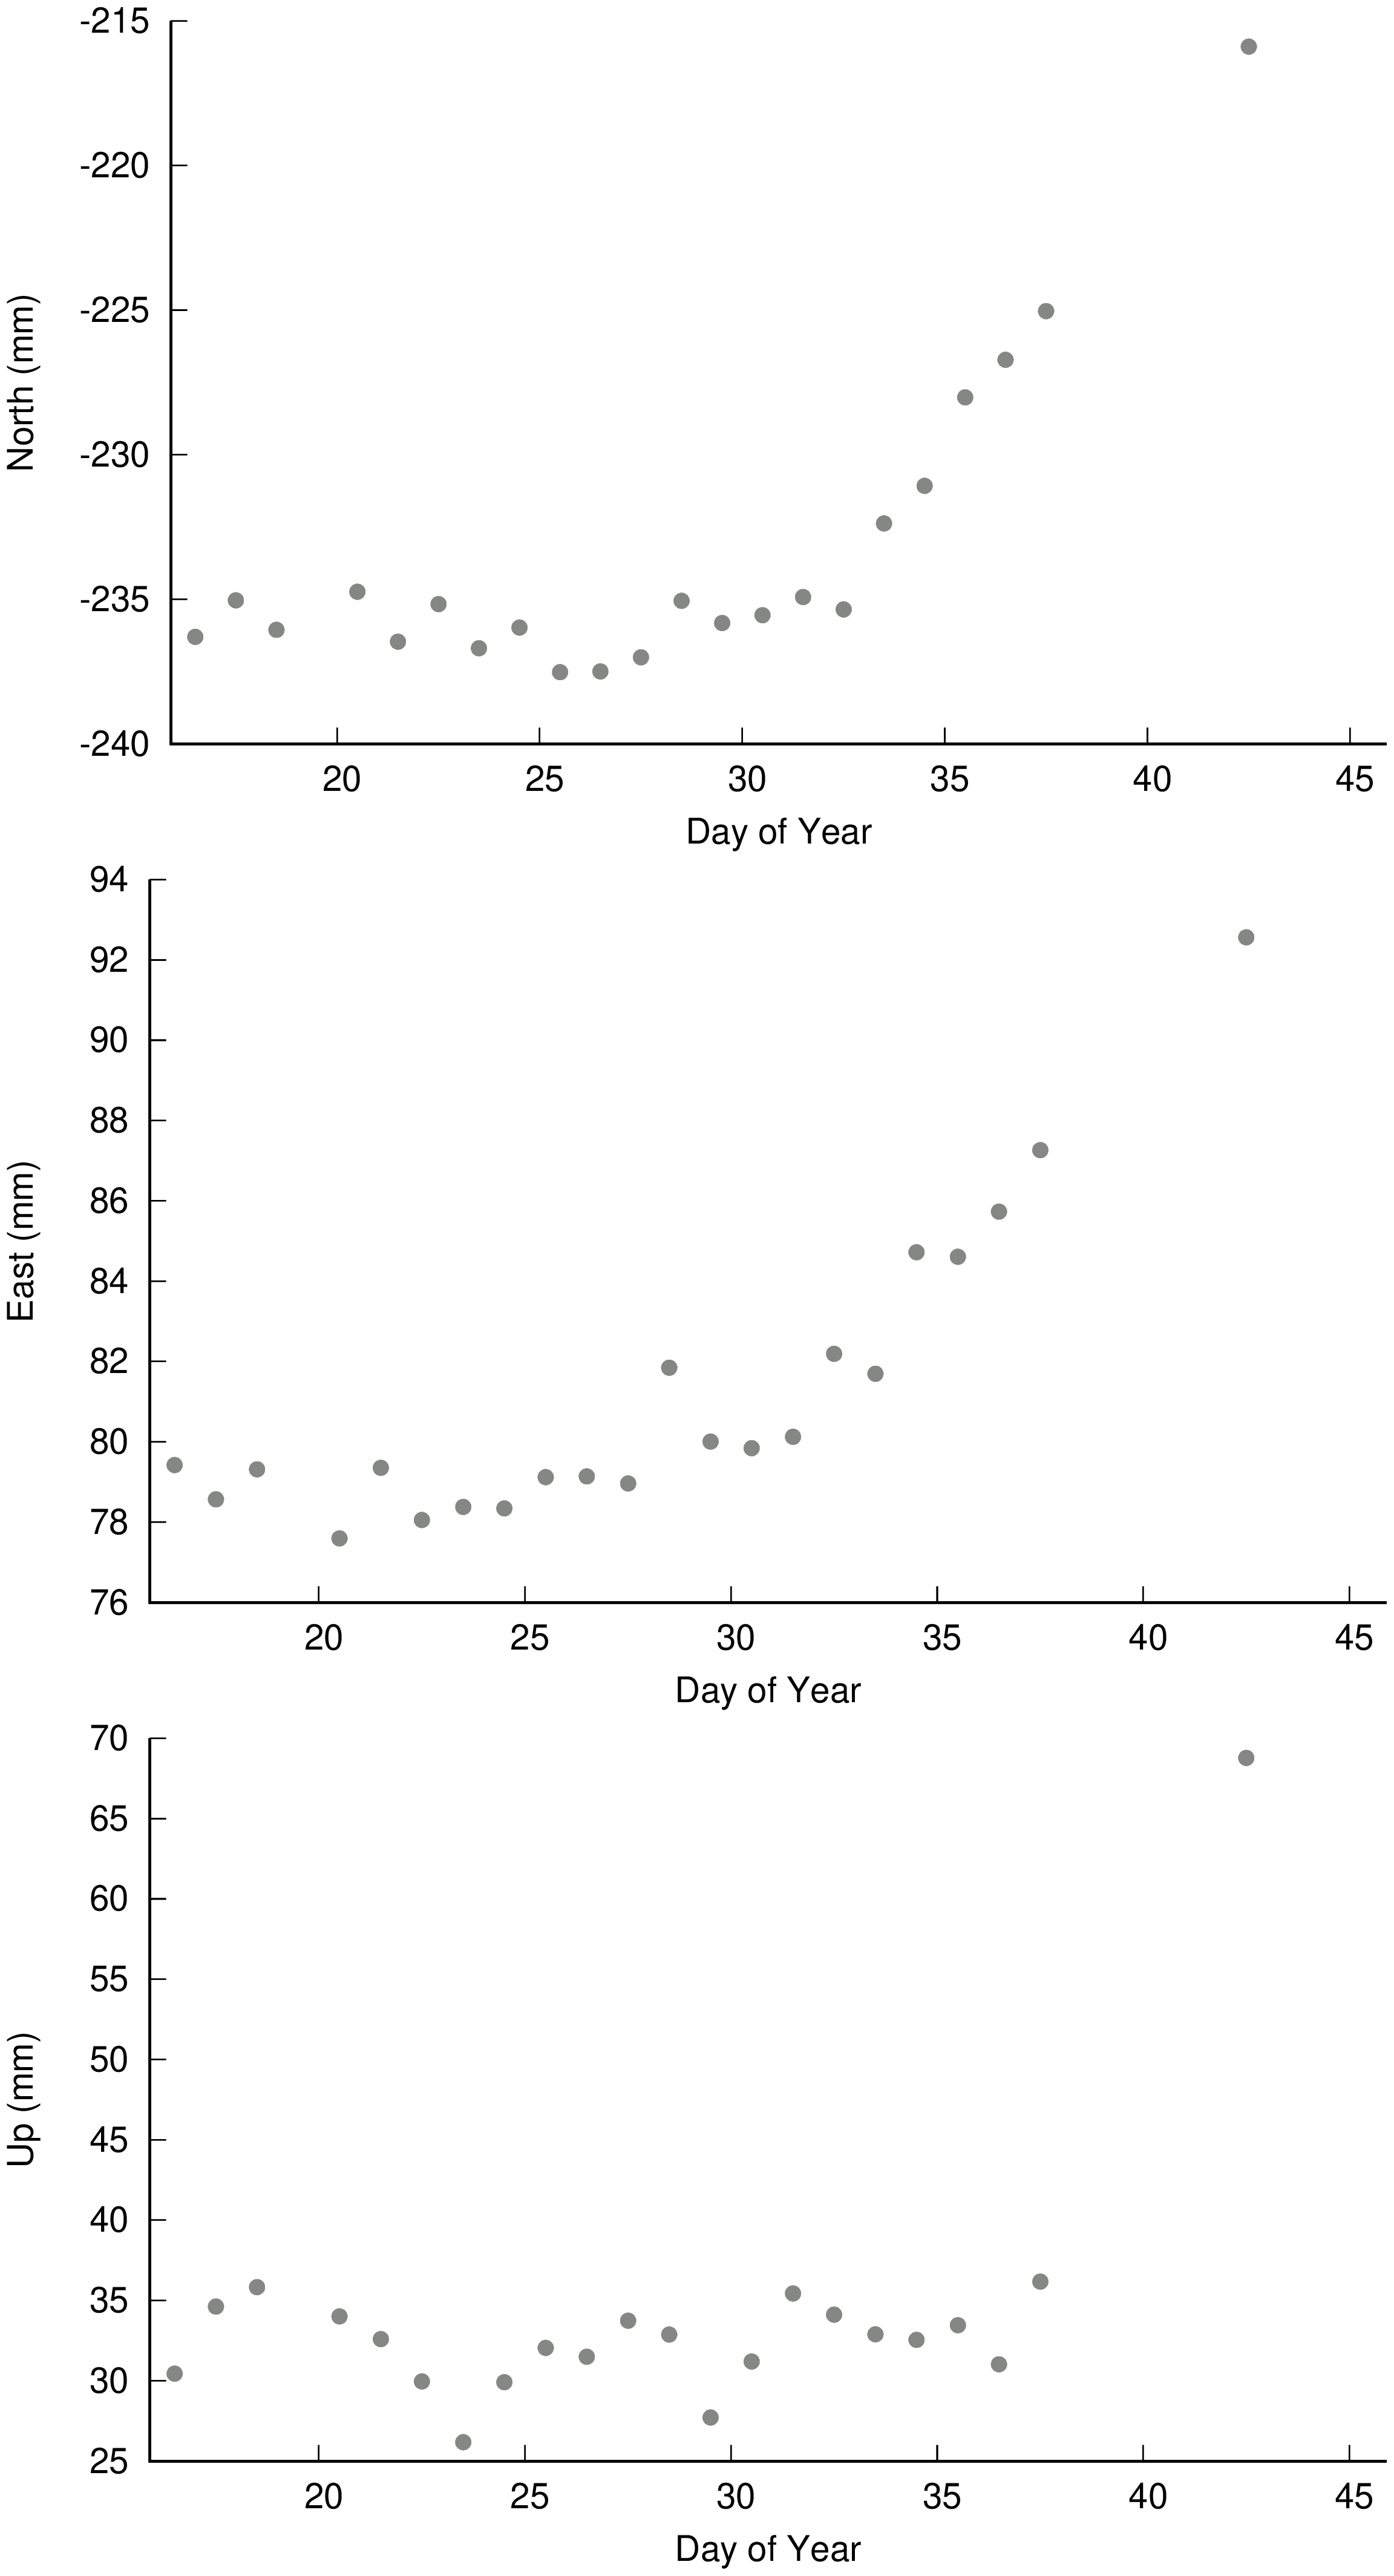
\includegraphics[width=.97\textwidth]{sntr-lmn.png}
      \end{center}       
    \end{column}
  \end{columns}  
  
\end{frame}
\note{}

 % ------------------------------------------------------------------------------
\begin{frame}
  \frametitle{Μετακινήσεις 2025 28/1 - 15/2 }
  \framesubtitle{}
  \label{}
  \vskip-.5cm
  \begin{columns}[T]
    \begin{column}{.5\textwidth}
      \begin{center}
        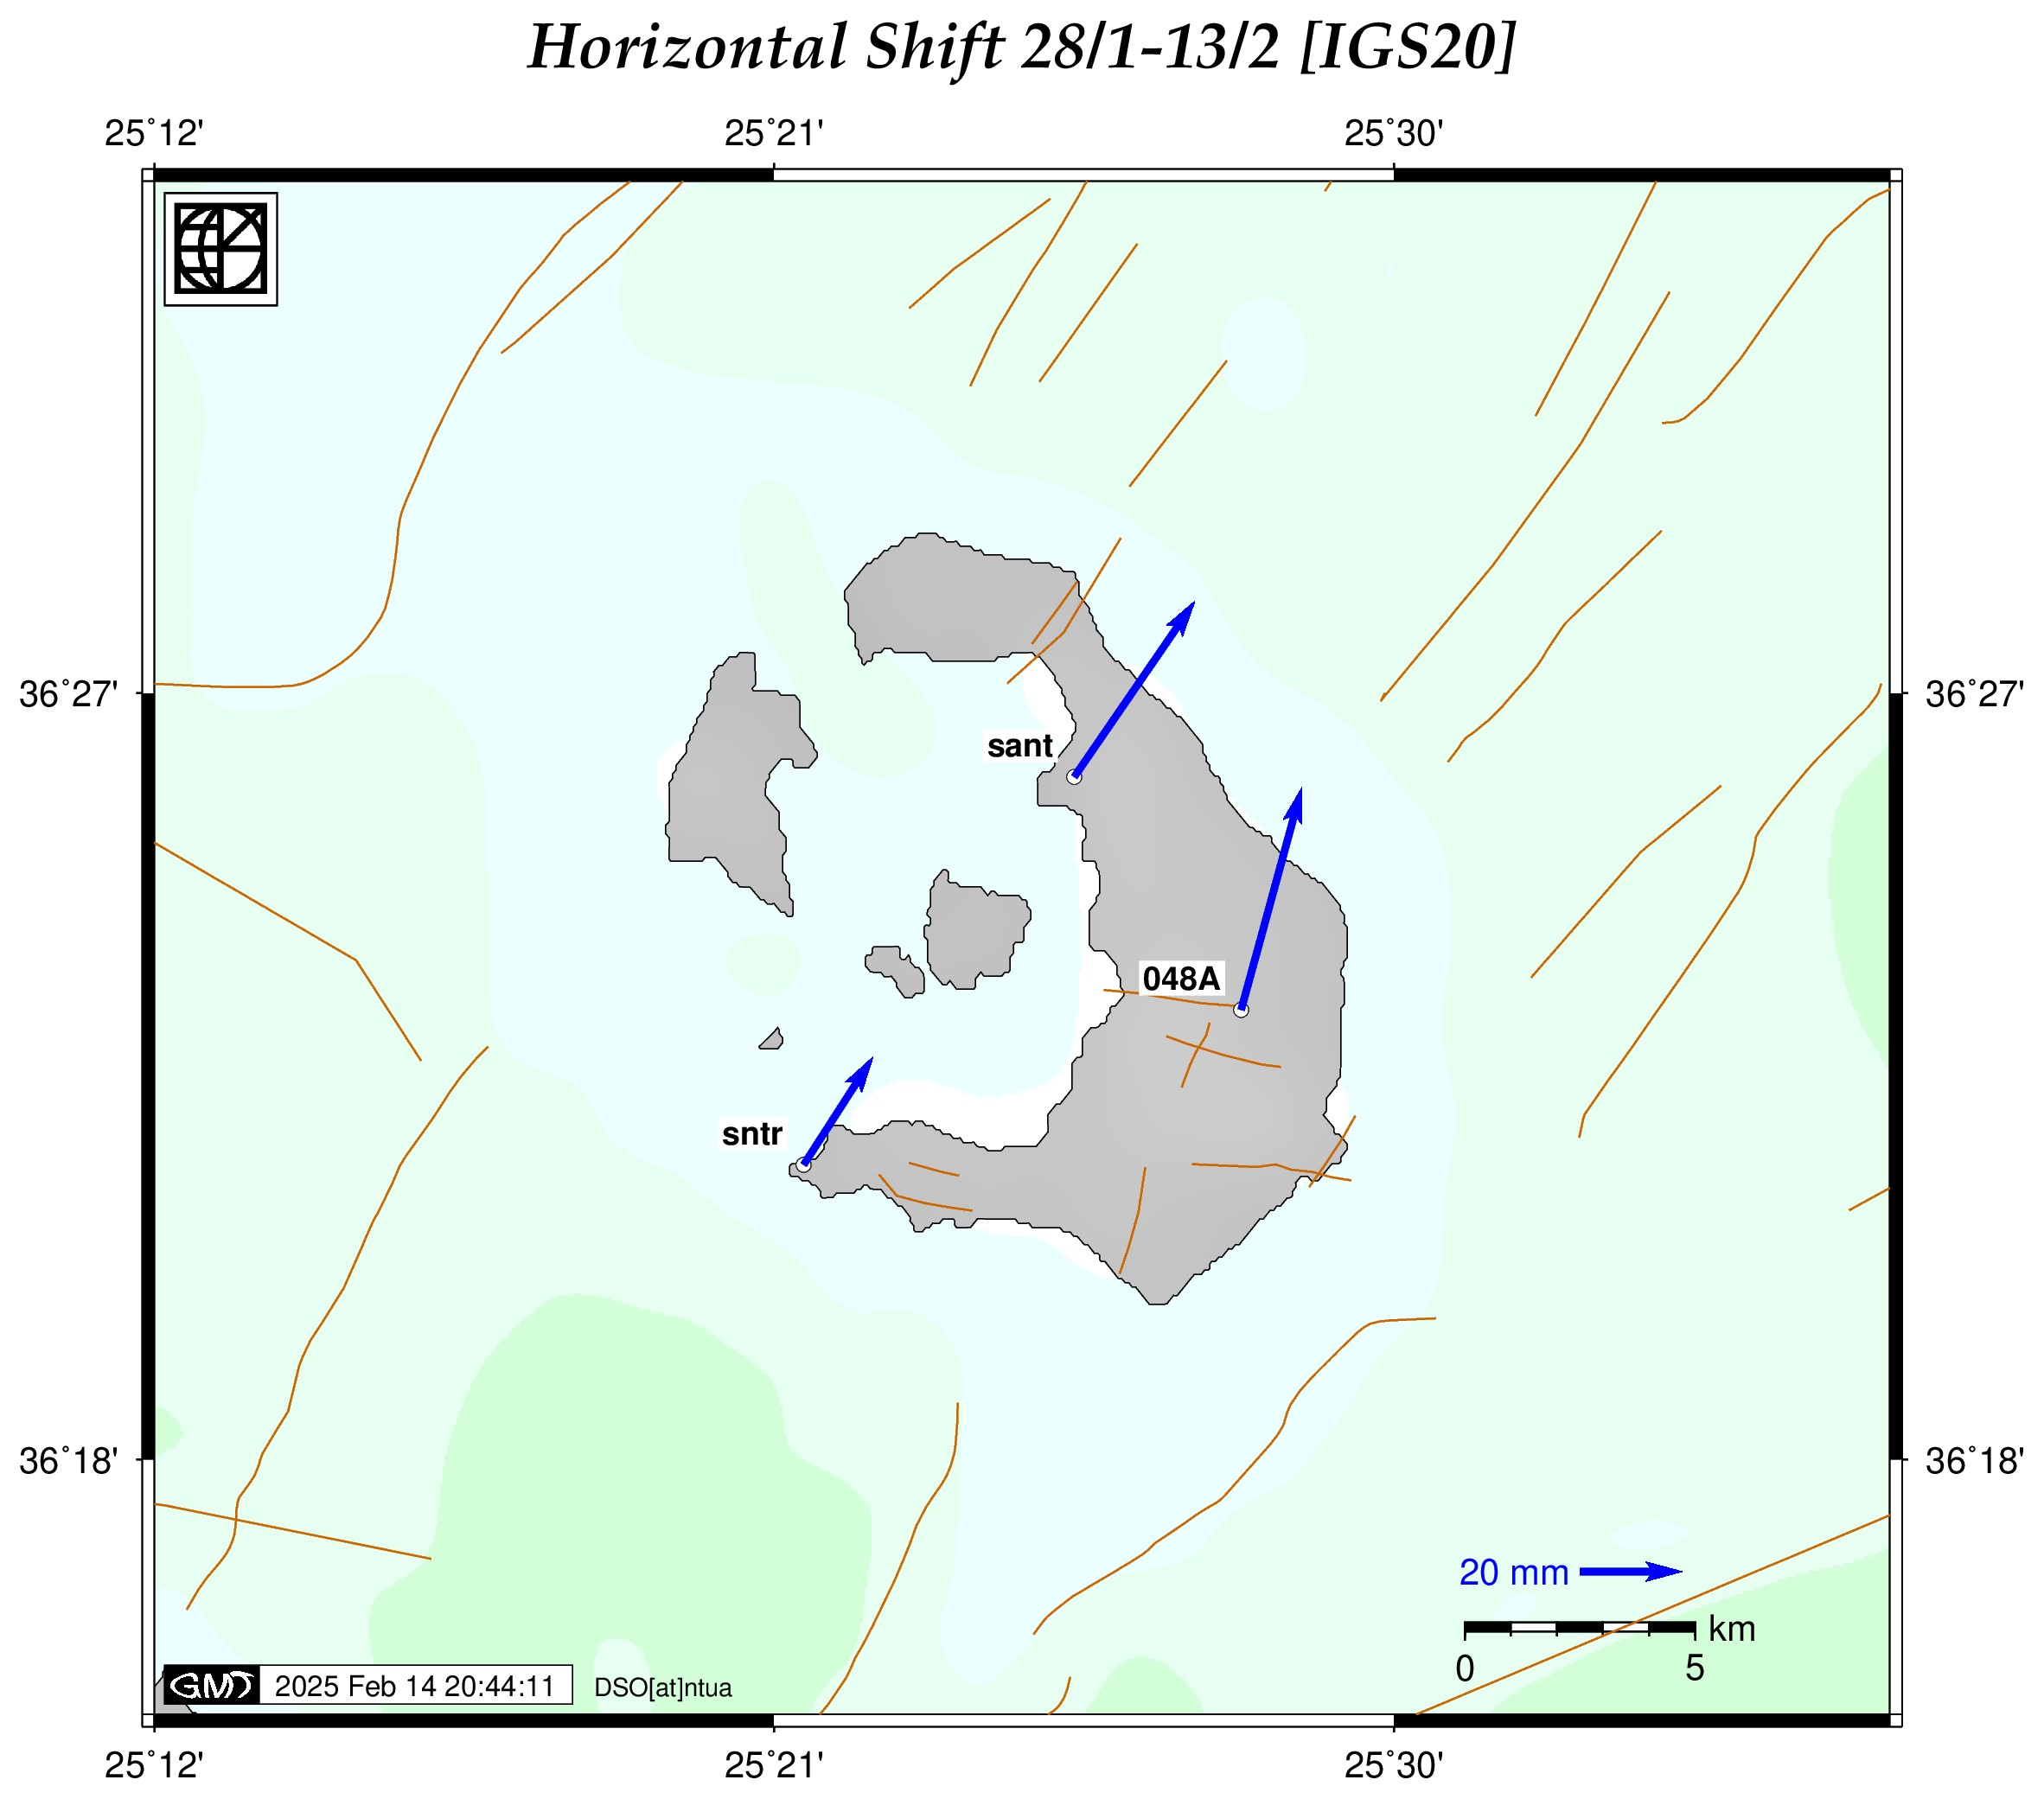
\includegraphics[width=.97\textwidth]{sant_2501_vhor.jpg}
      \end{center}  
    \end{column}
    \begin{column}{.5\textwidth}
      \begin{center}
        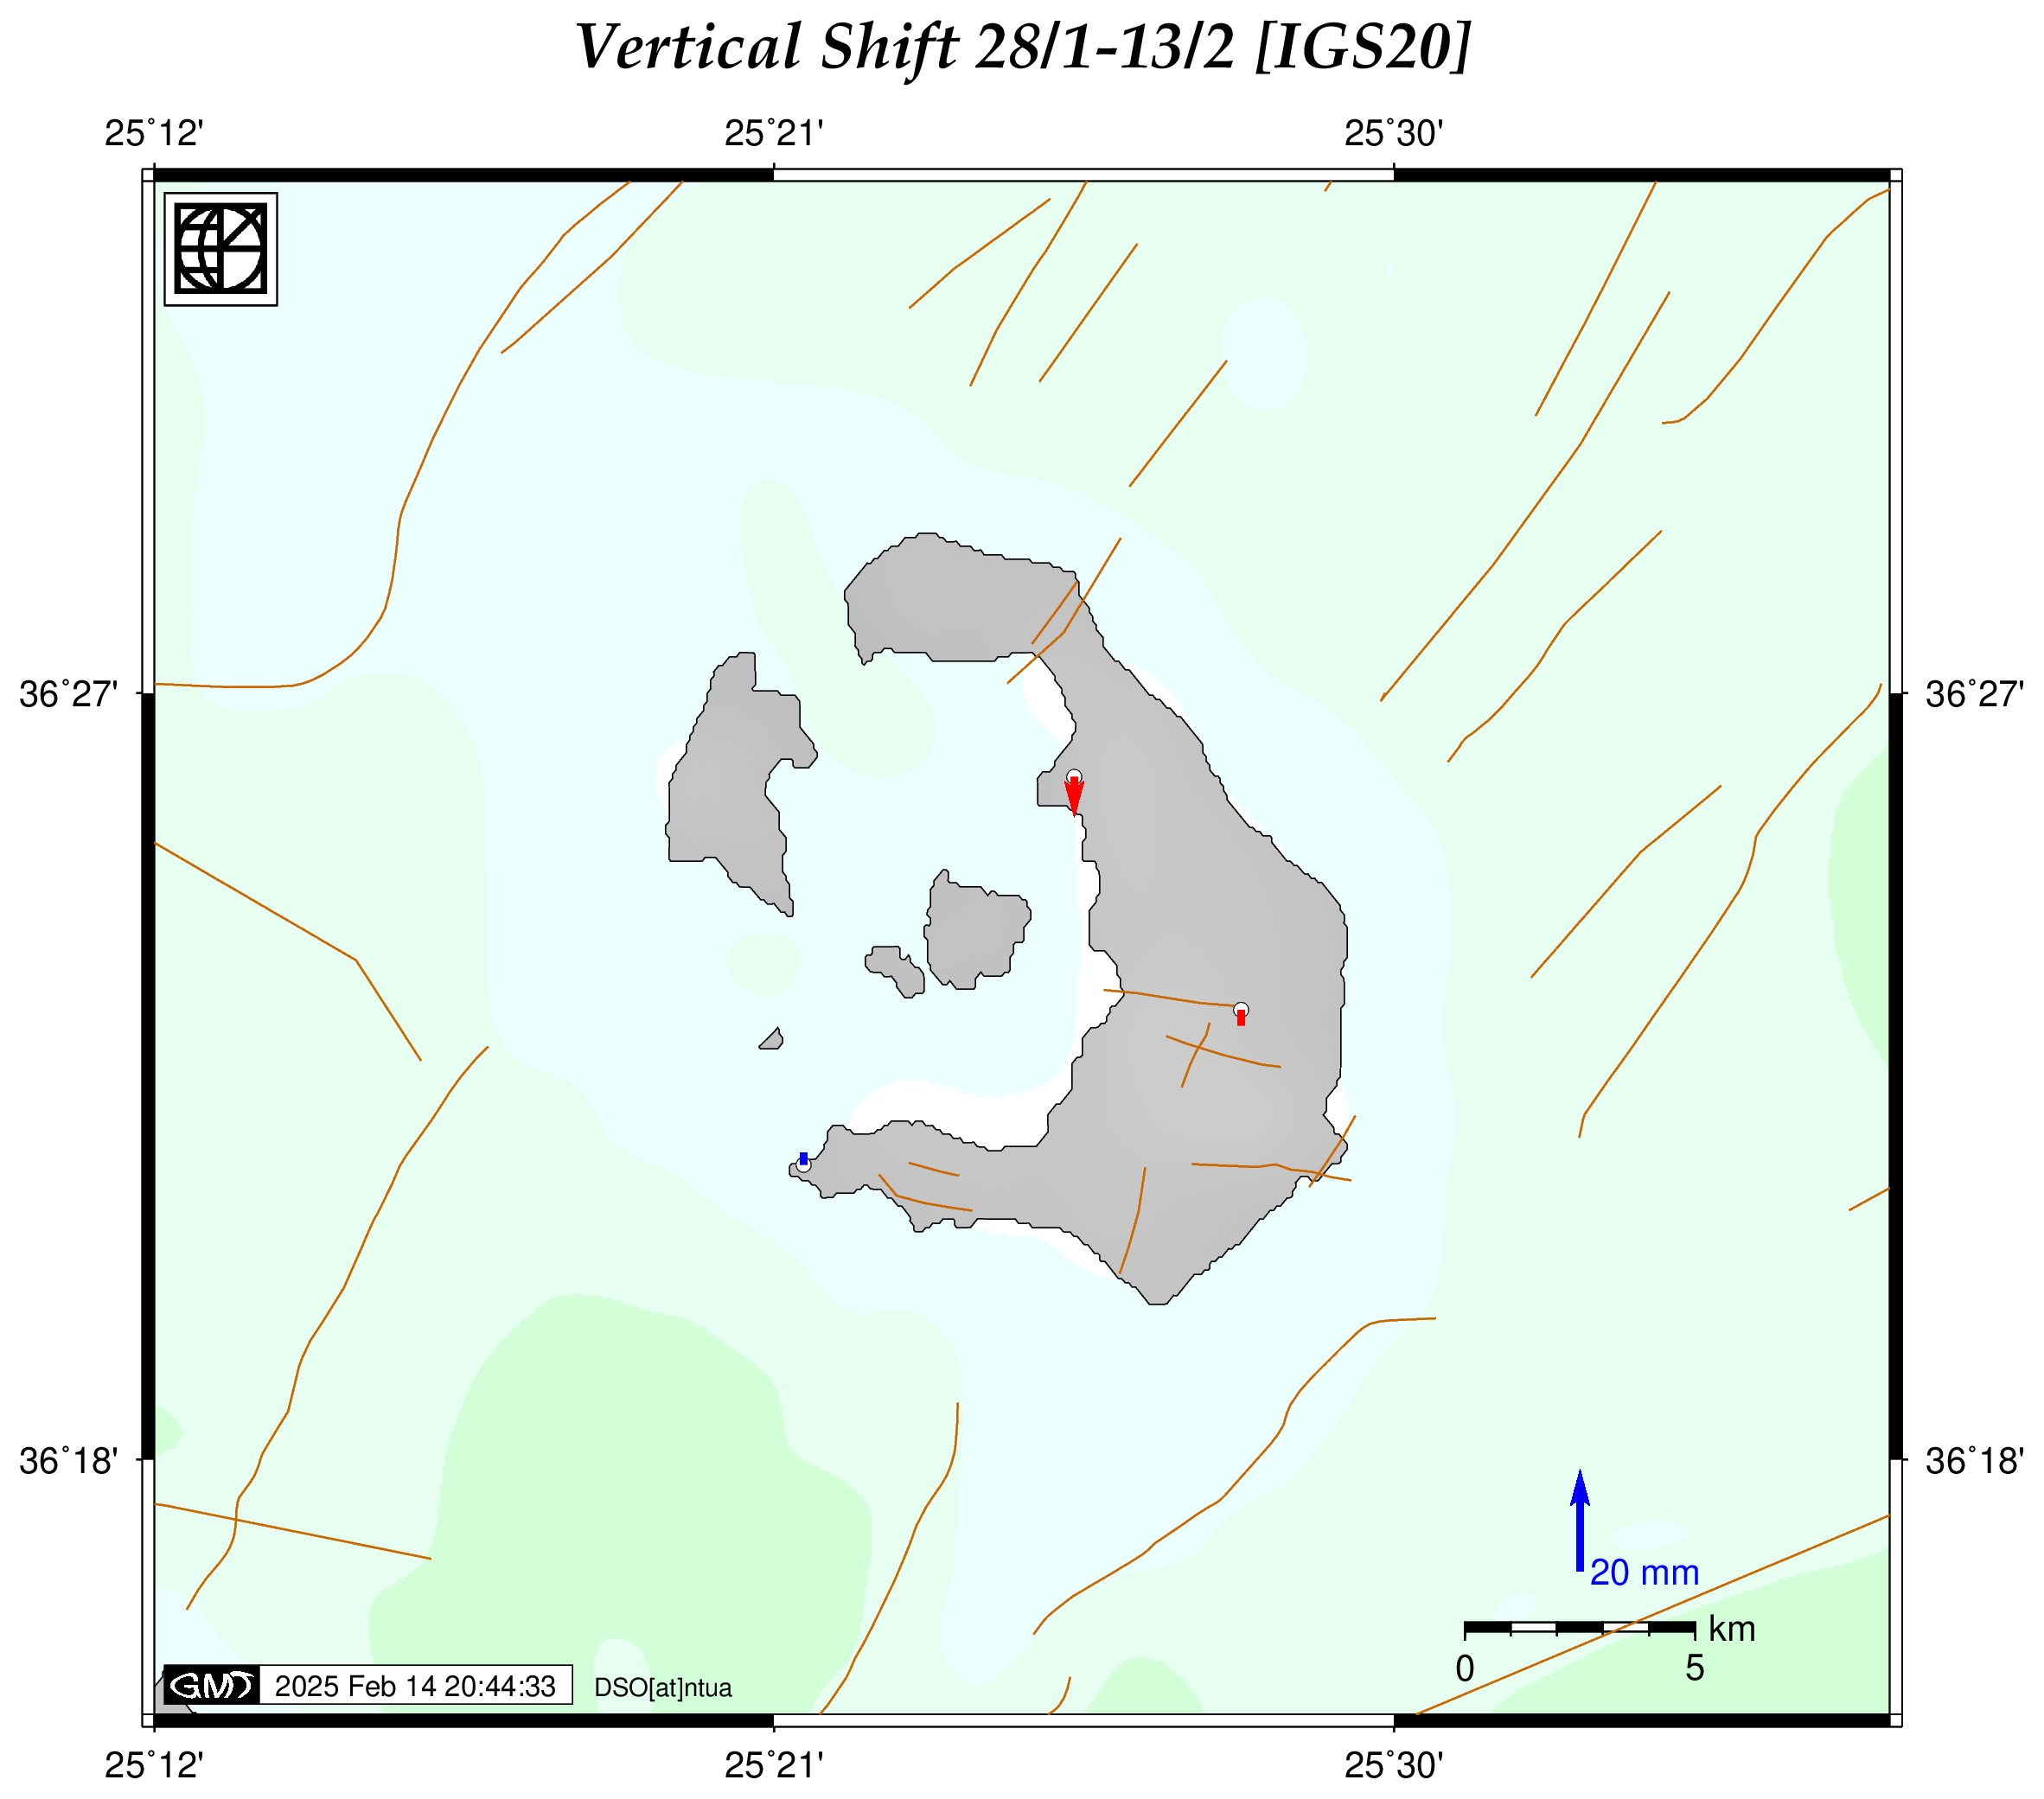
\includegraphics[width=.97\textwidth]{sant_2501_vver.jpg}
      \end{center}       
    \end{column}
  \end{columns}  

\end{frame}
\note{}

 % ------------------------------------------------------------------------------
\begin{frame}
  \frametitle{Μετακινήσεις 2025 28/1 - 15/2 }
  \framesubtitle{}
  \label{}
  \vskip-.5cm
  \begin{columns}[T]
    \begin{column}{.5\textwidth}
      \begin{center}
        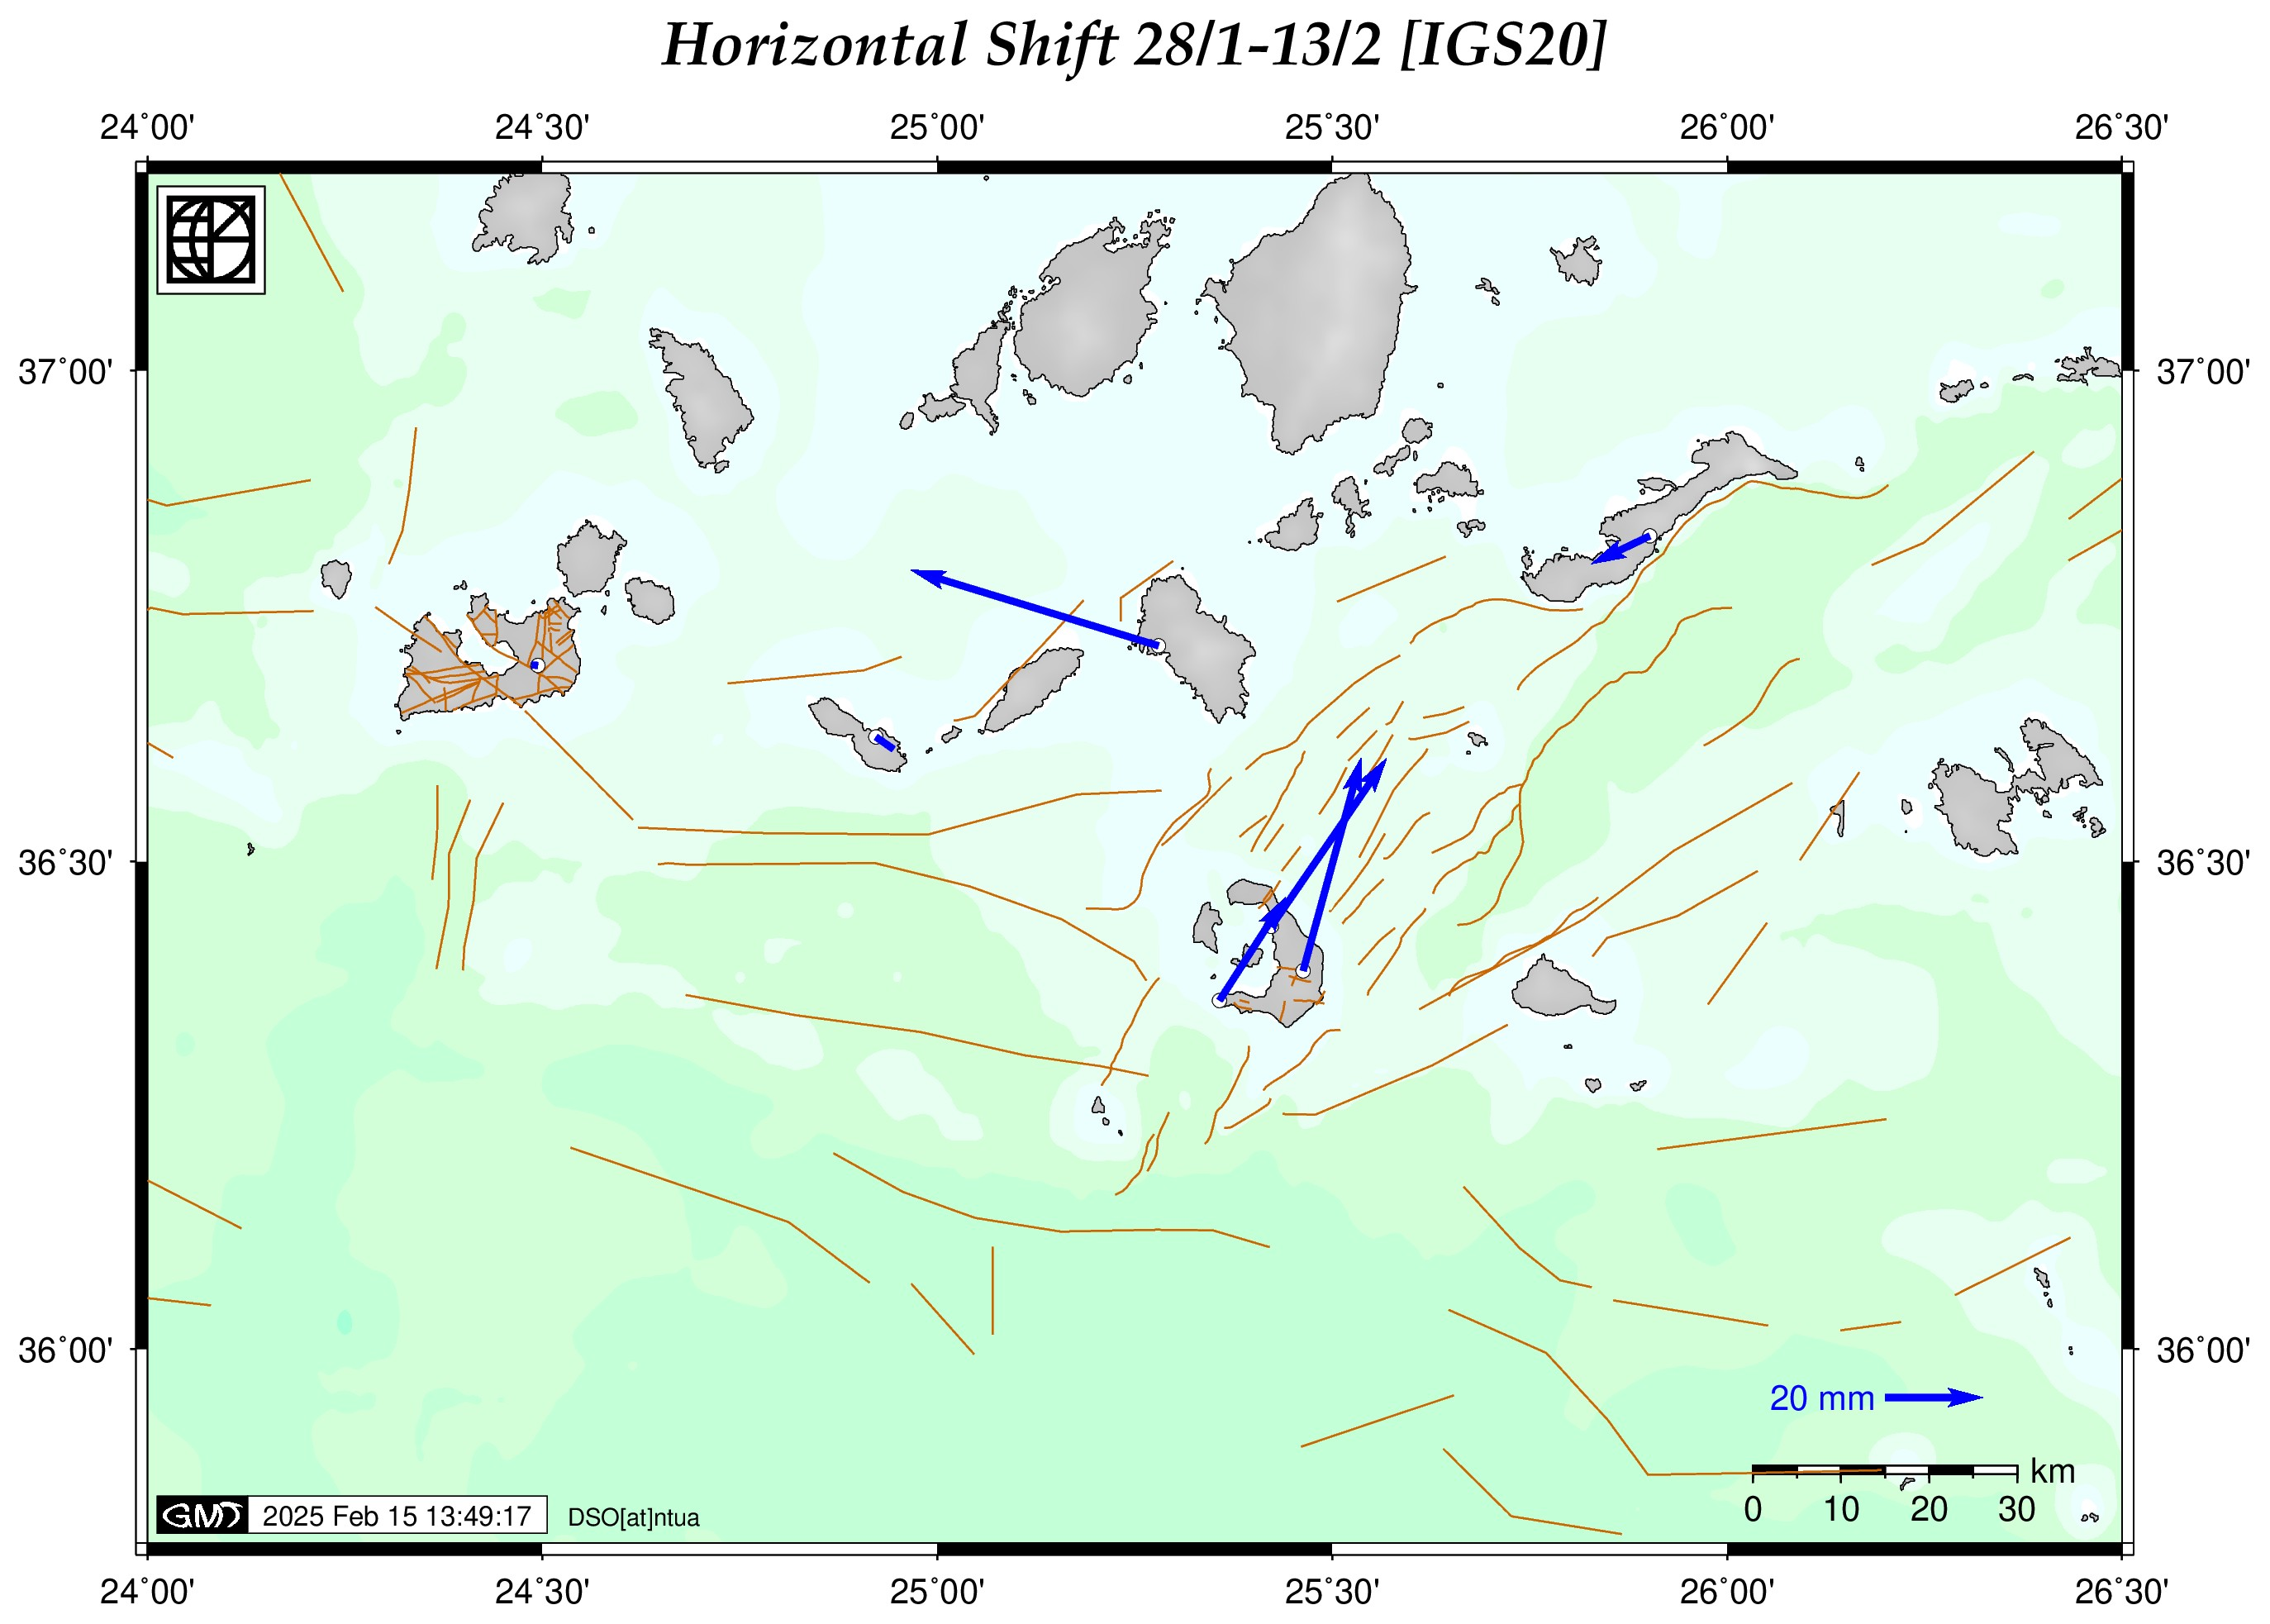
\includegraphics[width=.97\textwidth]{sant_2501_vhor01.jpg}
      \end{center}  
    \end{column}
    \begin{column}{.5\textwidth}
      \begin{center}
        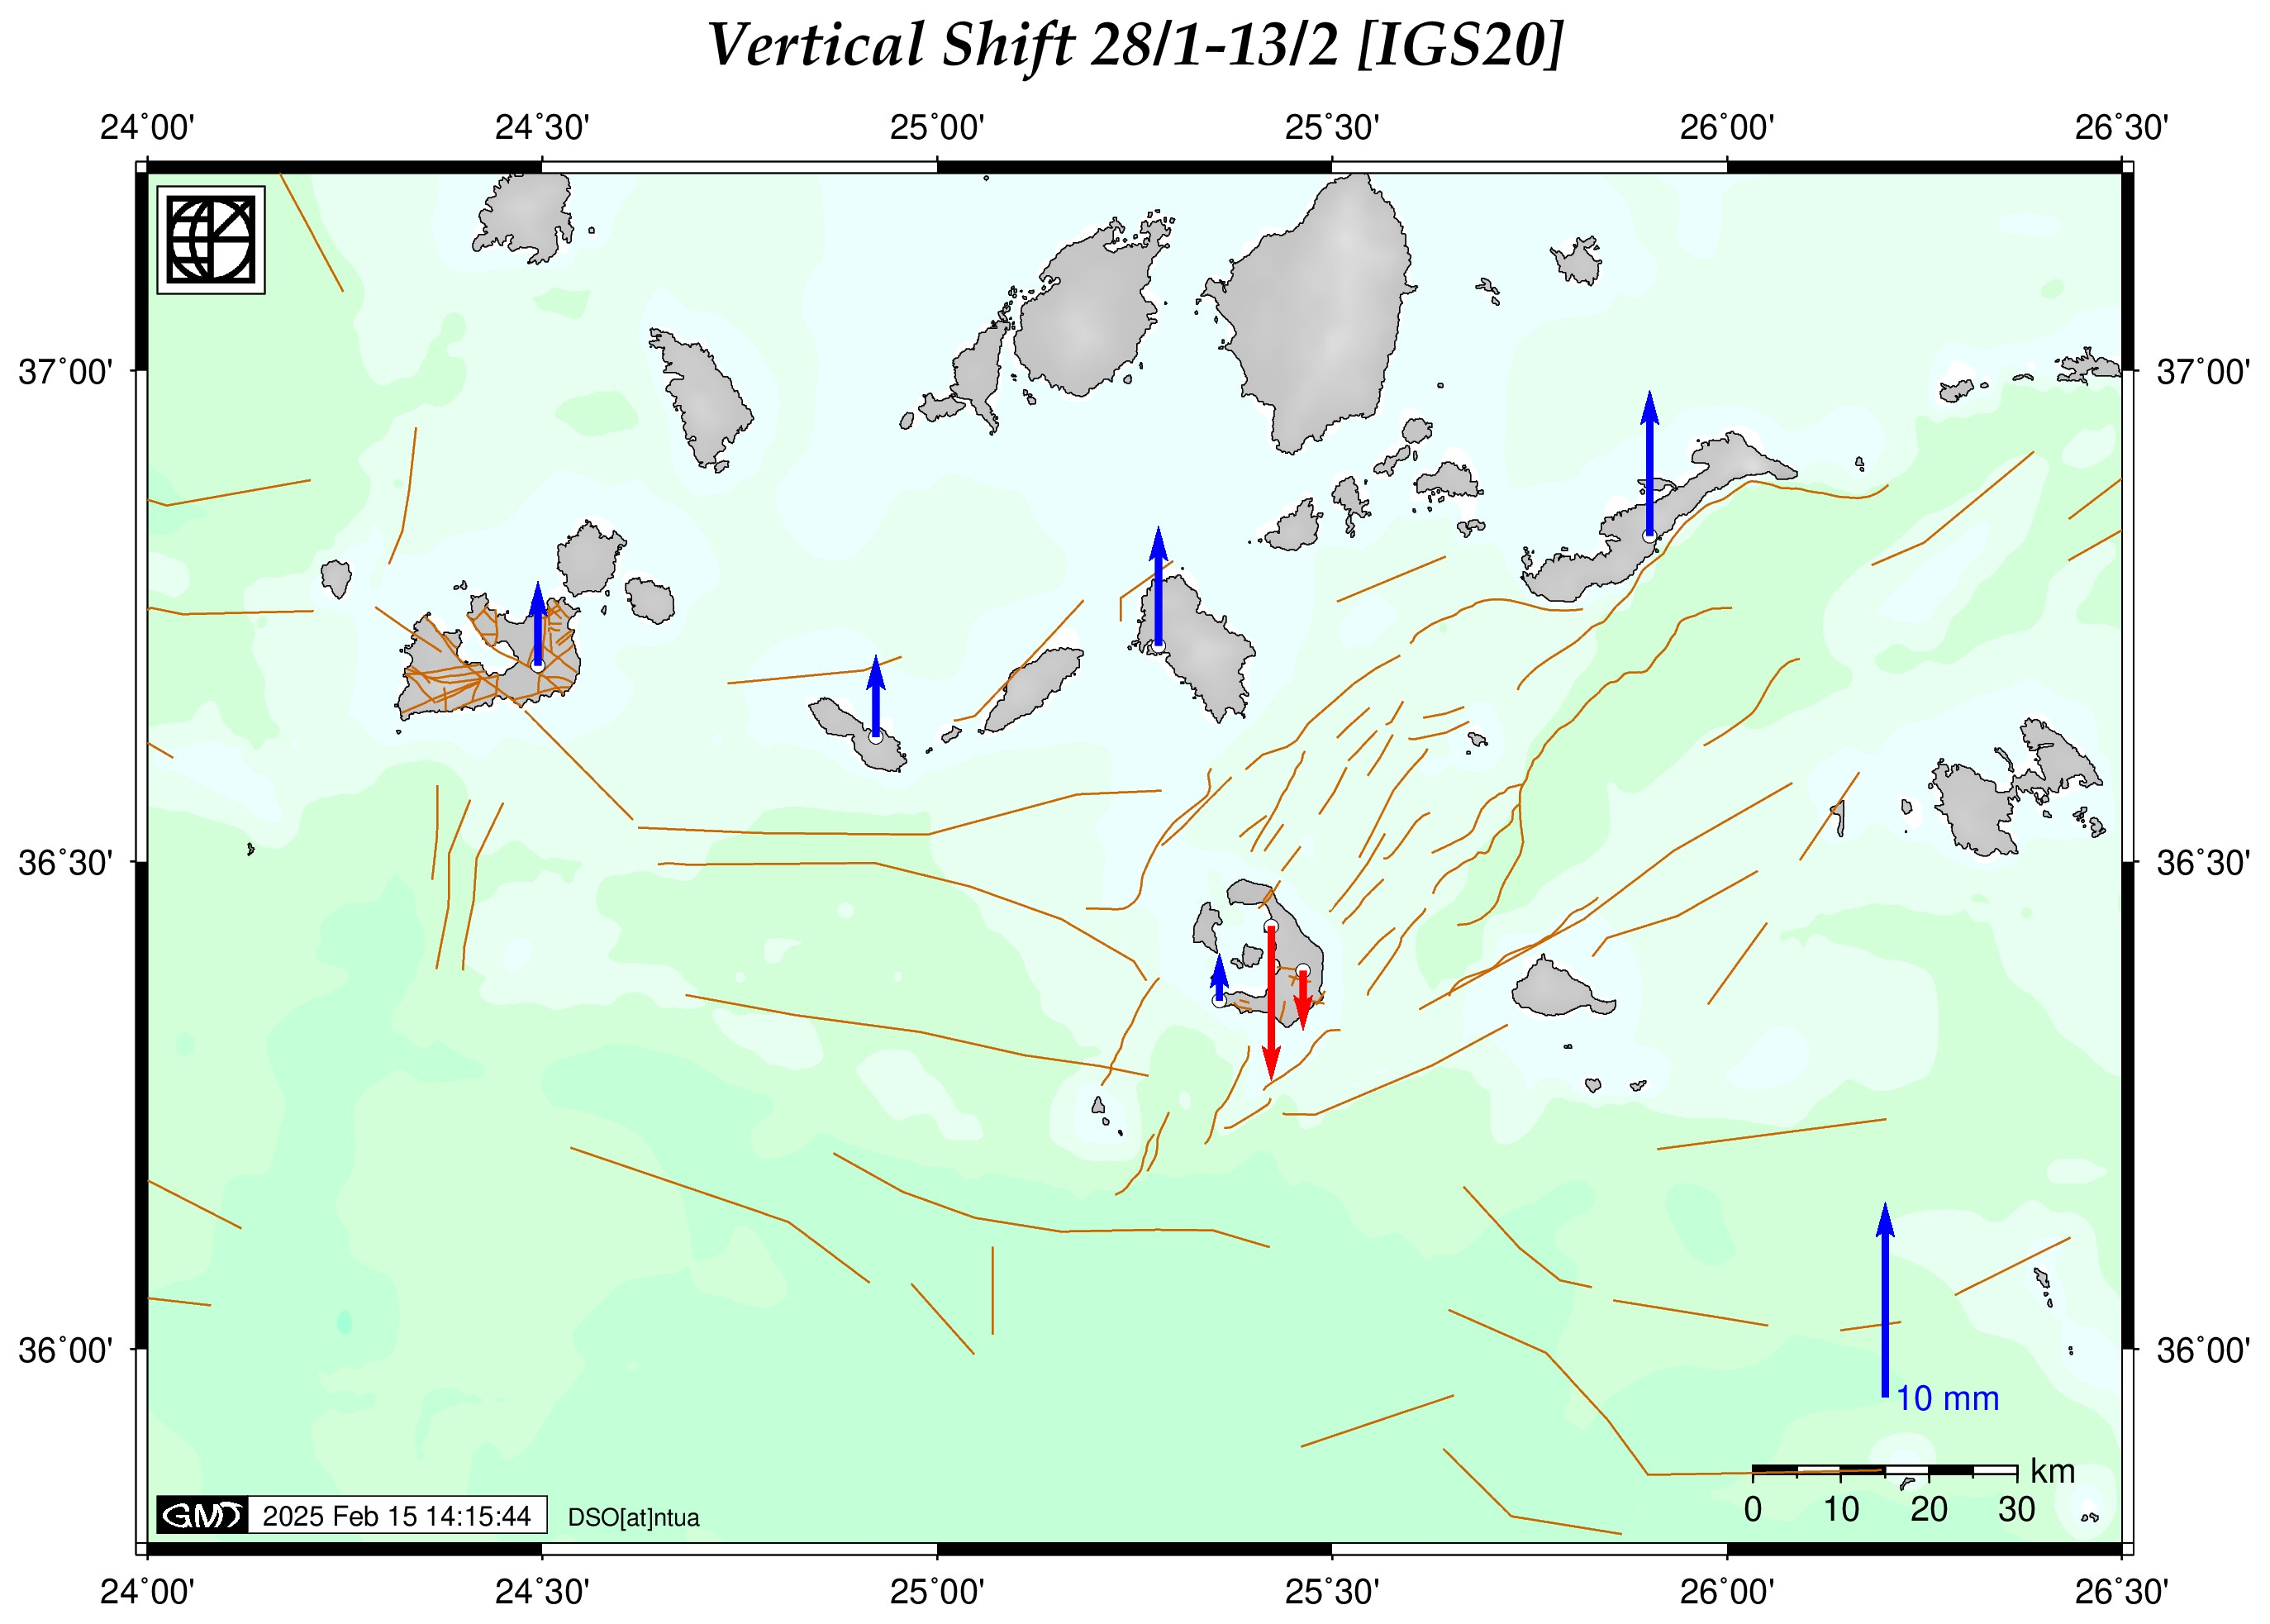
\includegraphics[width=.97\textwidth]{sant_2501_vver01.jpg}
      \end{center}       
    \end{column}
  \end{columns}  

\end{frame}
\note{}

 % ------------------------------------------------------------------------------
\begin{frame}
  \frametitle{Λειτουργία σταθμών}
  \framesubtitle{}
  \label{}
  \vskip-1cm
  \begin{columns}[T]
    \begin{column}{.25\textwidth}
      \begin{center}
      {\scriptsize SNTR 12653M001}
        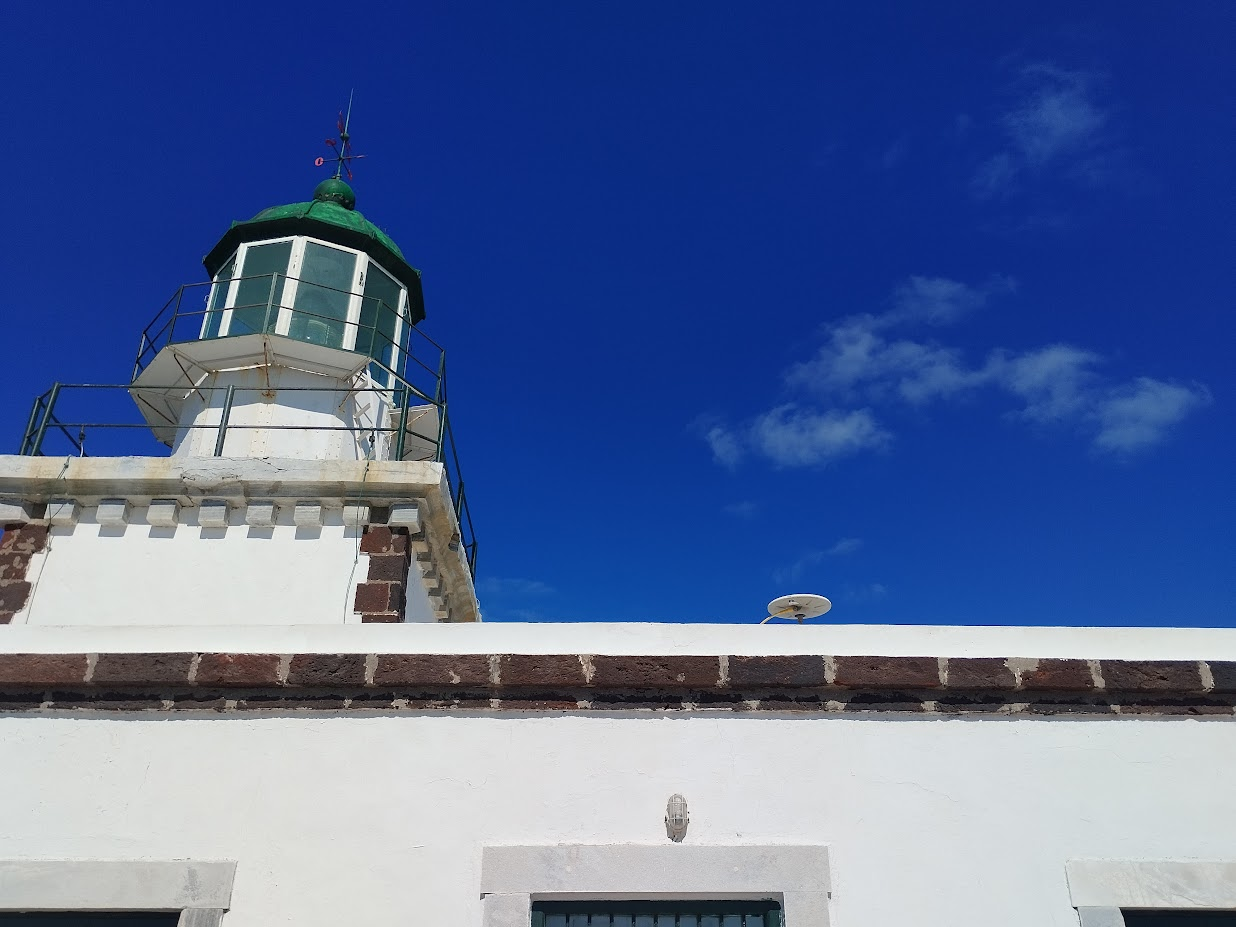
\includegraphics[width=.97\textwidth]{SNTR_01.jpg}
      \end{center}  
    \end{column}
    \begin{column}{.25\textwidth}
      \begin{center}
       {\scriptsize WNRY 12687M001}
        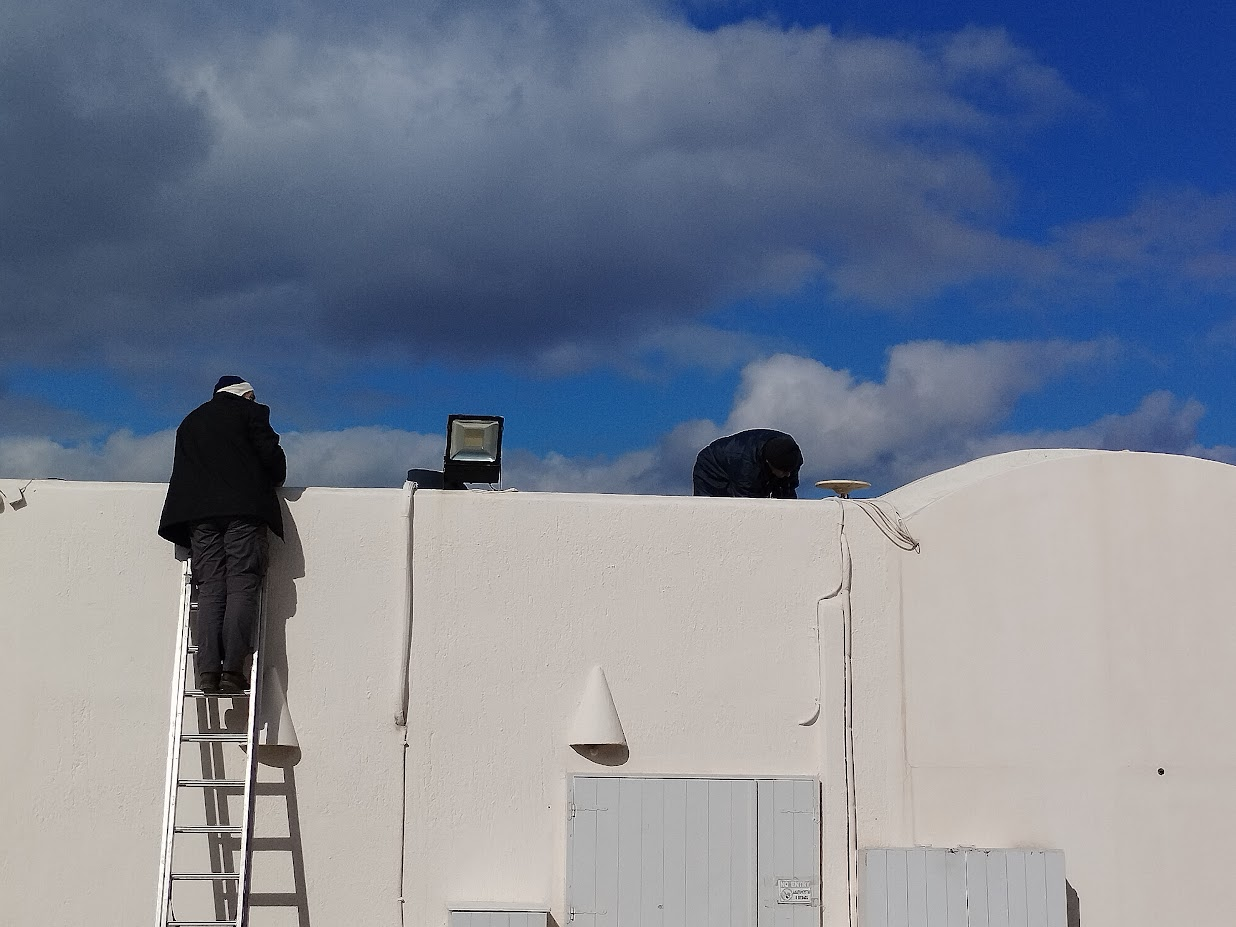
\includegraphics[width=.97\textwidth]{wnry_01.jpg}
      \end{center}       
    \end{column}
  \begin{column}{.25\textwidth}
      \begin{center}
       {\scriptsize NOMI}
        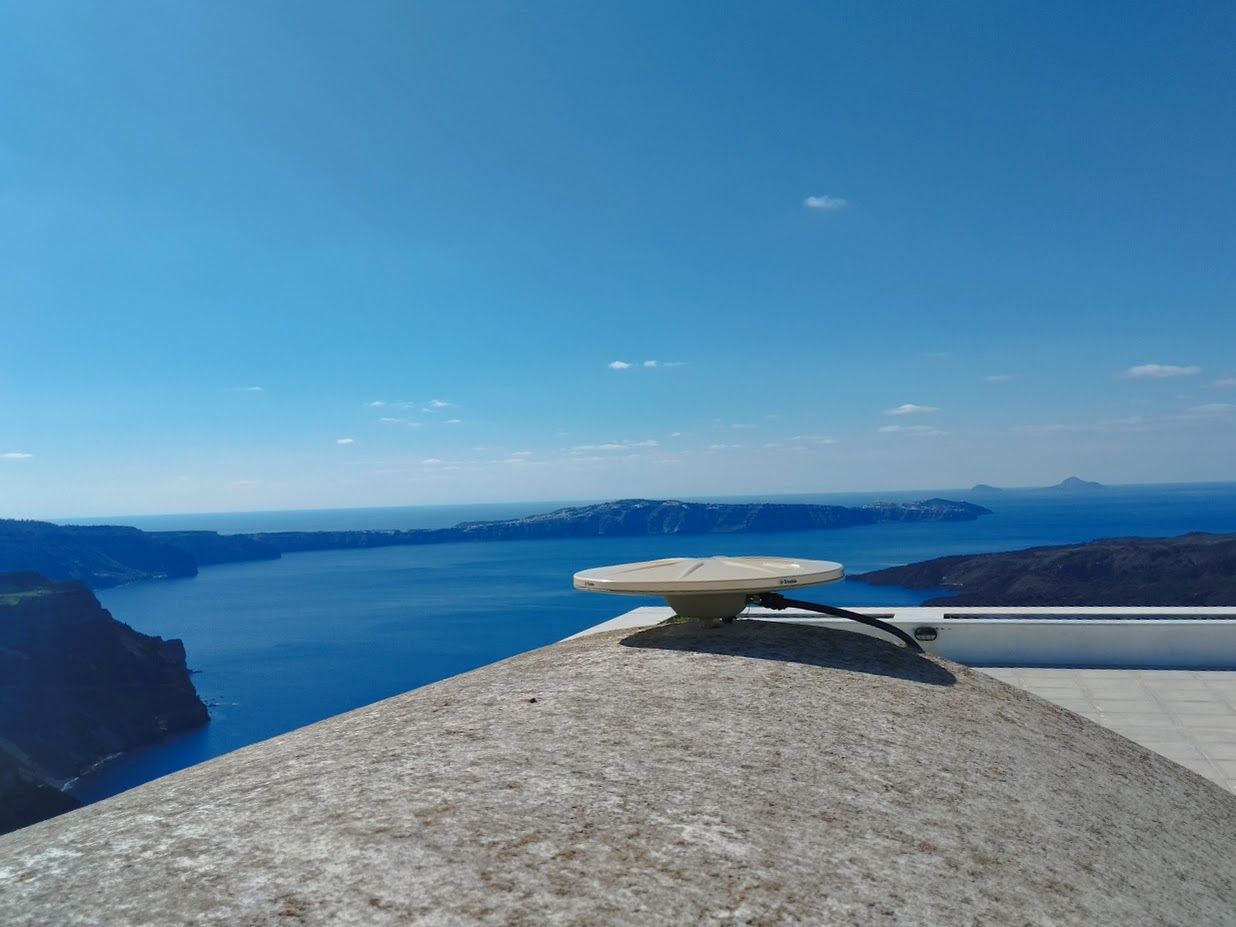
\includegraphics[width=.97\textwidth]{NOMI_01.jpg}
      \end{center}  
    \end{column}
    \begin{column}{.25\textwidth}
      \begin{center}
       {\scriptsize Campaign}
        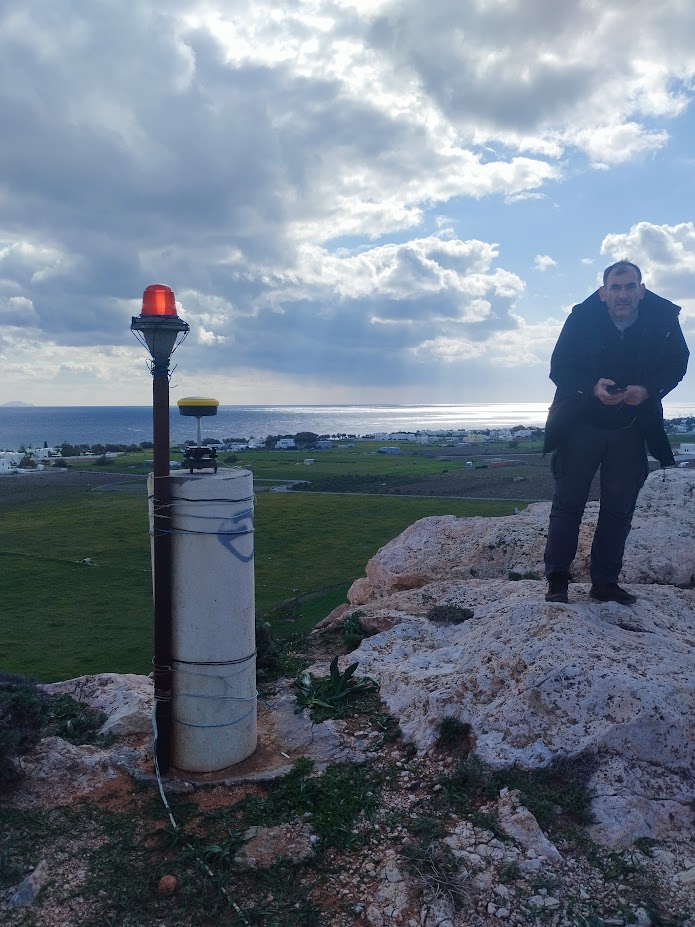
\includegraphics[width=.7\textwidth]{sn_camp.jpg}
      \end{center}       
    \end{column}
  \end{columns}  
  ~\\[1em]
\begin{scriptsize}
- Διάθεση δεδομένων: \url{http://dionysos.survey.ntua.gr/dsoportal/\_datacenter/httpdata.html}\\
- Ο σταθμός ΝΟΜΙ είναι σε συνεργασία με το Πανεπιστήμιο Πατρών και την άδεια του EarthScope.
\end{scriptsize}

\end{frame}
\note{}

 % ------------------------------------------------------------------------------
\begin{frame}
  \frametitle{Διάθεση δεδομένανων/αποτελεσμάτων}
  \framesubtitle{}
  \label{}
  \vskip-1.2cm
\begin{center}
  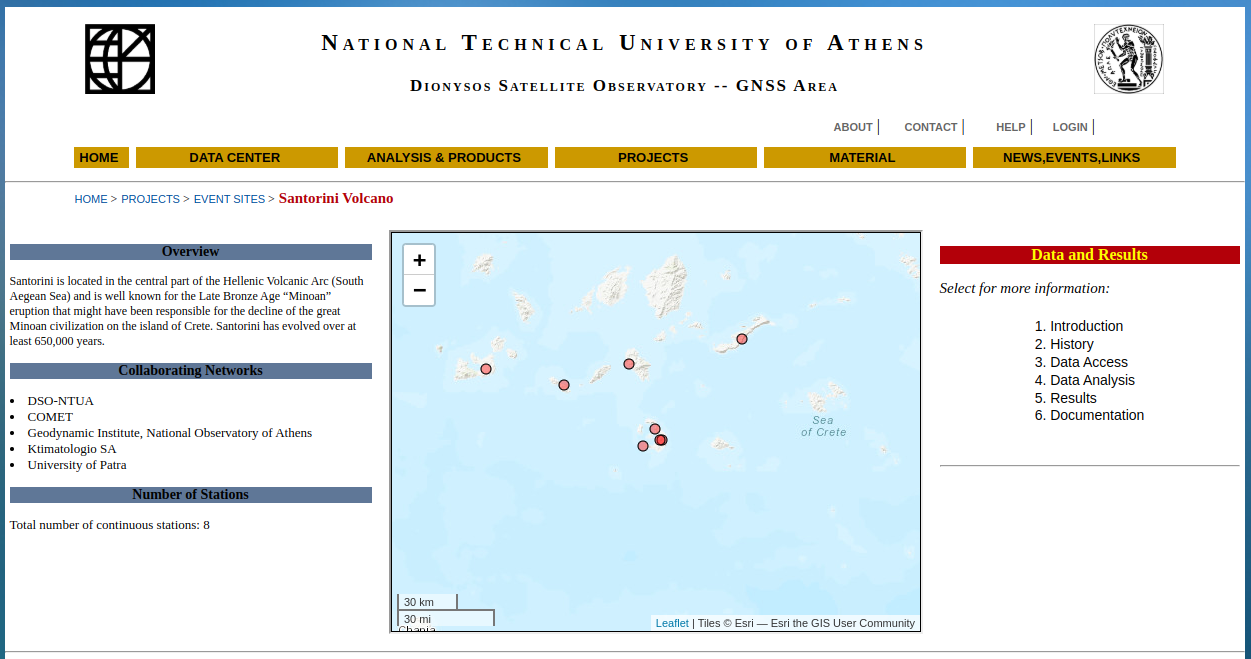
\includegraphics[width=.8\textwidth]{dsoportal_sant.png}
\end{center}
\url{http://dionysos.survey.ntua.gr/dsoportal/\_projects/supersites/santorini/}
\end{frame}
\note{}